\section{\textcolor{red}{Performance Evaluation}}
\label{sec:perf}

%zhu begin

In this section, we validated the effectiveness of our methods, including features extraction, users clustering and reposting behavior modeling.

\subsubsection{Experimental Setup}

The data we used in this study was crawled from Sina Microblog, which allows users to follow with each other. When user A follows B, A is called the follower of B and B is called the friend of A. User B's behaviors such as posting and reposting will be visible to A. User A can choose microblogs to repost which was posted (or reposted) by user B. Our data set was crawled by the following ways. Firstly, we selected 43500 users randomly from the public Microblog stream. We crawled the basic information of these users, including gender, province, number of microblogs, city, number of followers, number of friends, signature, nickname, etc. In addition, we also crawled all the microblogs the user posted or reposted. The microblog information including the number of it has been reposted, the number of it has been commented, the number of it has been liked, type of the microblog (be posted or reposted by the user), the location where the microblog was posted, the content of the microblog, the device the microblog was posted by, the time when the microblog was posted and so on. In addition, we can get part of one user's friends from the microblogs that user reposted. So we also collected some users's friends's information and microblogs. Table \ref{tab:Data_statistics} lists the statistics information of the data set. Another dataset we used here was 1000 labeled microblogs selected from the microblogs we crawled. We labeled each microblog with categories in the cell lexicon.\par

\begin{table}[!h]
\centering
    \caption{statistics information of Dataset }     % NOTE!  caption goes _before_ the table contents !!
    \label{tab:Data_statistics}
    \begin{small}
    \begin{tabular}{|l|l|l|l|l|}
    \hline
    \cline{2-5}
    {\bfseries DataSet} & {\bfseries  \#Users}         & {\bfseries \#Microblogs}     & {\bfseries \#Posts}    & {\bfseries \#Reposts}     \\
    \hline
    WeiBo         & 410000 & 157943530		& 77234797 & 80708733	\\
    \hline
    \end{tabular}
    \end{small}
\end{table}

\paragraph{Features Extraction}
One user's basic and behavioral information can be obtained either from the data set straightly or from the statistics information of user's microblogs. As for user's interests, we proposed a novel method to do interest extraction. Here we compared our method using different parameters with method that just using TF-IDF or Twitter-LDA. To evaluate the performance of the method, we labeled 1000 microblogs with categories of the cell lexicon. One microblog may belong to one or several categories. Considering it's a multi-label problem, our evaluation metrics here are accuracy, precision and recall as described in \cite{IEEEexample:journals/tkde/ZhangZ14}. Let $S = {(x_i,Y_i)| 1 \le i \le p)}$ be the test set and $m(\cdot)$ be the mapping method. The accuracy, precision and recall are defined as equation \eqref{accuracy_m}, \eqref{precision_m} and \eqref{recall_m}.\par

\begin{equation}\label{accuracy_m}
accuracy_m = \frac{1}{p} \sum_{i=1}^{p} \frac{\mid Y_i \cap m(x_i) \mid}{\mid Y_i \cup m(x_i) \mid}
\end{equation}

\begin{equation}\label{precision_m}
precision_m = \frac{1}{p} \sum_{i=1}^{p} \frac{\mid Y_i \cap m(x_i) \mid}{\mid m(x_i) \mid}
\end{equation}

\begin{equation}\label{recall_m}
recall_m = \frac{1}{p} \sum_{i=1}^{p} \frac{\mid Y_i \cap m(x_i) \mid}{\mid Y_i \mid}
\end{equation}

\paragraph{Users Clustering}
We used the data generated by features extraction to perform users clustering. Each sample contains user's basic features, behavioral features and interests features. Silhouette coefficient \cite{IEEEexample:books/mk/HanKP2011} was used as our evaluation metric here. For each sample $i$, let $a(i)$ be the average dissimilarity of $i$ with all other data within the same cluster. Let $b(i)$ be the lowest average dissimilarity of $i$ to any other cluster, of which $i$ is not a member. We now get the silhouette of sample $i$ as equation \eqref{silhouetteOfi}. Then silhouette coefficient of the result with N samples can be got as equation \eqref{silhouette}.\par

\begin{equation}\label{silhouetteOfi}
s(i) = \frac{b(i)-a(i)}{max\{b(i),a(i)\}}
\end{equation}

\begin{equation}\label{silhouette}
silhouette = \frac{1}{N} \sum_{i=1}^{N} s(i)
\end{equation}

\paragraph{Reposting Behavior Modeling}
For analyzing reposting behavior, we firstly divided users into groups by users clustering. For each group, we randomly selected microblogs reposted by users of the group as positive samples, and selected microblogs ,which were reposted by a friend of one user in the group but not reposted by this user, as negative samples. Then we generated final samples with features described in subsection \ref{subsec:RepostingBehaviorPrediction}. We have carefully chosen algorithm to compare with our method. Here we compared our method with \cite{IEEEexample:conf/ijcai/ZhangLTCL13}, which studied a state-of-art idea of social influence locality for modeling users¡¯ reposting behaviors in the microblog network. We use accuracy, recall and f-measure as our evaluation metrics.\par

All experiments were conducted on a machine with 2 Intel Xeon E5¨C2630 2.4GHz CPUs and 64 GB of Memory, running 64 bit Windows 7 professional system. Each experiment was repeated 5 times, and the average is reported here. In all the experiments, we fixed parameters to their default values. The parameters with their descriptions and default values are presented in Table \ref{tab:Parameters}. \par

\begin{table}[!h]
\centering
    \caption{Parameters used in the experiments with their descriptions.  }
    % NOTE!  caption goes _before_ the table contents !!
    \label{tab:Parameters}
    \begin{small}
    \begin{tabular}{|c|l|c|}
    \hline
    {\bfseries Parameters} & {\bfseries  Descriptions}                       & {\bfseries Default}     \\
    \hline
                       & threshold for selecting                             & \\
    $\epsilon$         & the categories when considering                     & 3\\
                       & the number of overlapped words.                     & \\
    \hline
                       & weight for mapping value                            & \\	
    $\alpha$           & by performing Procedure 1                           & 0.7\\
    \hline
                       & threshold number for                                & \\
    $k$                & selecting categories when                           & 3\\
                       & performing mapping algorithm.                       &	\\
    \hline
    $k_1$              & min number of clusters                              & 2	\\
    \hline
    $k_2$              & max number of clusters                              & 10	\\
    \hline
    \end{tabular}
    \end{small}
\end{table}


\subsubsection{Performance and Analysis}


\paragraph{Features Extraction}

To accurately extract user's interests feature, we proposed a novel method that combined the method of Twitter-LDA \cite{IEEEexample:zhao2011comparing} and TF-IDF to tag the microblog with 512 categories. We performed an experiment to compare three methods which only using Twitter-LDA, only using TF-IDF, and combining the two with different value of $\alpha$. Fig \ref{fig:Interests} shows the results of the experiment. From the results, we can see that when combining the two, we got a better performance. We also developed a demo system for visualization of users's features, fig. \ref{fig:userFeatures} shows one case of a user.

\begin{comment}
\begin{figure}[h]
	\centerline{\psfig{figure=IMAGE/features/Interests.eps,height=50.54mm,width=82mm}}
	\caption{Visualization for User Features.}
	\label{fig:Interests}
\end{figure}
\end{comment}

\begin{figure}[!htb]
\centering
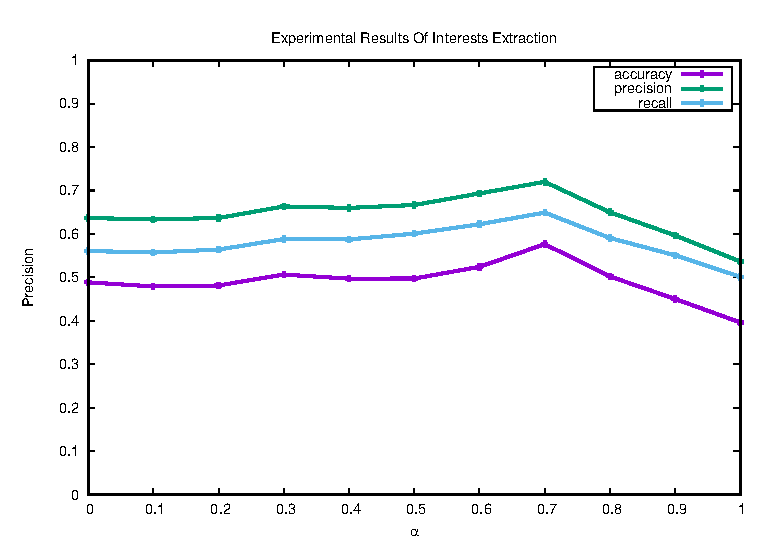
\includegraphics[width=.96\linewidth]{IMAGE/features/Interests}
\caption{Visualization for User Features.}
\label{fig:Interests}
\end{figure}


\begin{comment}
\begin{figure}[h]
	\centerline{\psfig{figure=IMAGE/features/userfeatures.eps,height=120.54mm,width=92mm} }
	\caption{Visualization for User Features.}
	\label{fig:userFeatures}
\end{figure}
\end{comment}

\begin{figure}[!htb]
\centering
\includegraphics[width=.96\linewidth]{IMAGE/features/userfeatures}
\caption{Visualization for User Features.}
\label{fig:userFeatures}
\end{figure}

\paragraph{User Clustering}

We performed users clustering on the 43500 users we selected through the method described in subsection \ref{subsec:UserClustering}. In addition, we reconstructed five datasets which were randomly selected from the 43500 users and each dataset had 10000 users. The results are list in Fig. \ref{fig:sample_clustering}. From the results, we can draw the following observations:
(1) On the whole dataset with 43500 users, the clustering method got its largest coefficient when the number of clusters was four.
(2) On the five datasets with 10000 users, the clustering method got its largest coefficient on four datasets when the number of clusters is four and one dataset when the number of clusters is three. Based on the observations, we thought it a reasonable result dividing 43500 users into four groups.\par


We carefully analyzed the four groups we obtained through users clustering. (1)Most of users of the group one are male, and they are mainly distributed in Beijing. What's more, most of these users have similar amount of friends and followers. The most active time of this group are mainly distributed between 10 am and 12 am. (2)The users of group two are mostly female, they are also mainly distributed in Beijing. Most of users also have similar amount of friends and followers as group one. The most active time of this group are mainly distributed between 22 pm and 24 pm. (3)The users of group three are mostly male, and they are distributed in a wide range of provinces. Most of users have the number of followers far more than friends. Users of this group are active both in 10-12 am and 22-24 pm. (4)Most of users of group four are female, and they are distributed in a wide range of provinces as group three. Most of these users have the number of followers far more than friends. And the most active time of this group are mainly distributed between 22 pm and 24 pm. We also found that the distribution of the number of users's microblogs of each group is similar. We visualized the users's interests using words cloud, the difference between groups is obvious, excepting that group one and group three have similar interests.

\begin{comment}
\begin{figure}[h]
	\centerline{\psfig{figure=IMAGE/clustering/Clustering.eps,width=80.7mm} }
	\caption{The Results of Users Clustering Performed on Six Datasets}
	\label{fig:sample_clustering}
\end{figure}
\end{comment}

\begin{figure}[!htb]
\centering
\includegraphics[width=.96\linewidth]{IMAGE/clustering/Clustering}
\caption{The Results of Users Clustering Performed on Six Datasets}
\label{fig:sample_clustering}
\end{figure}

\begin{figure}
  \centering
  \subfigure{
      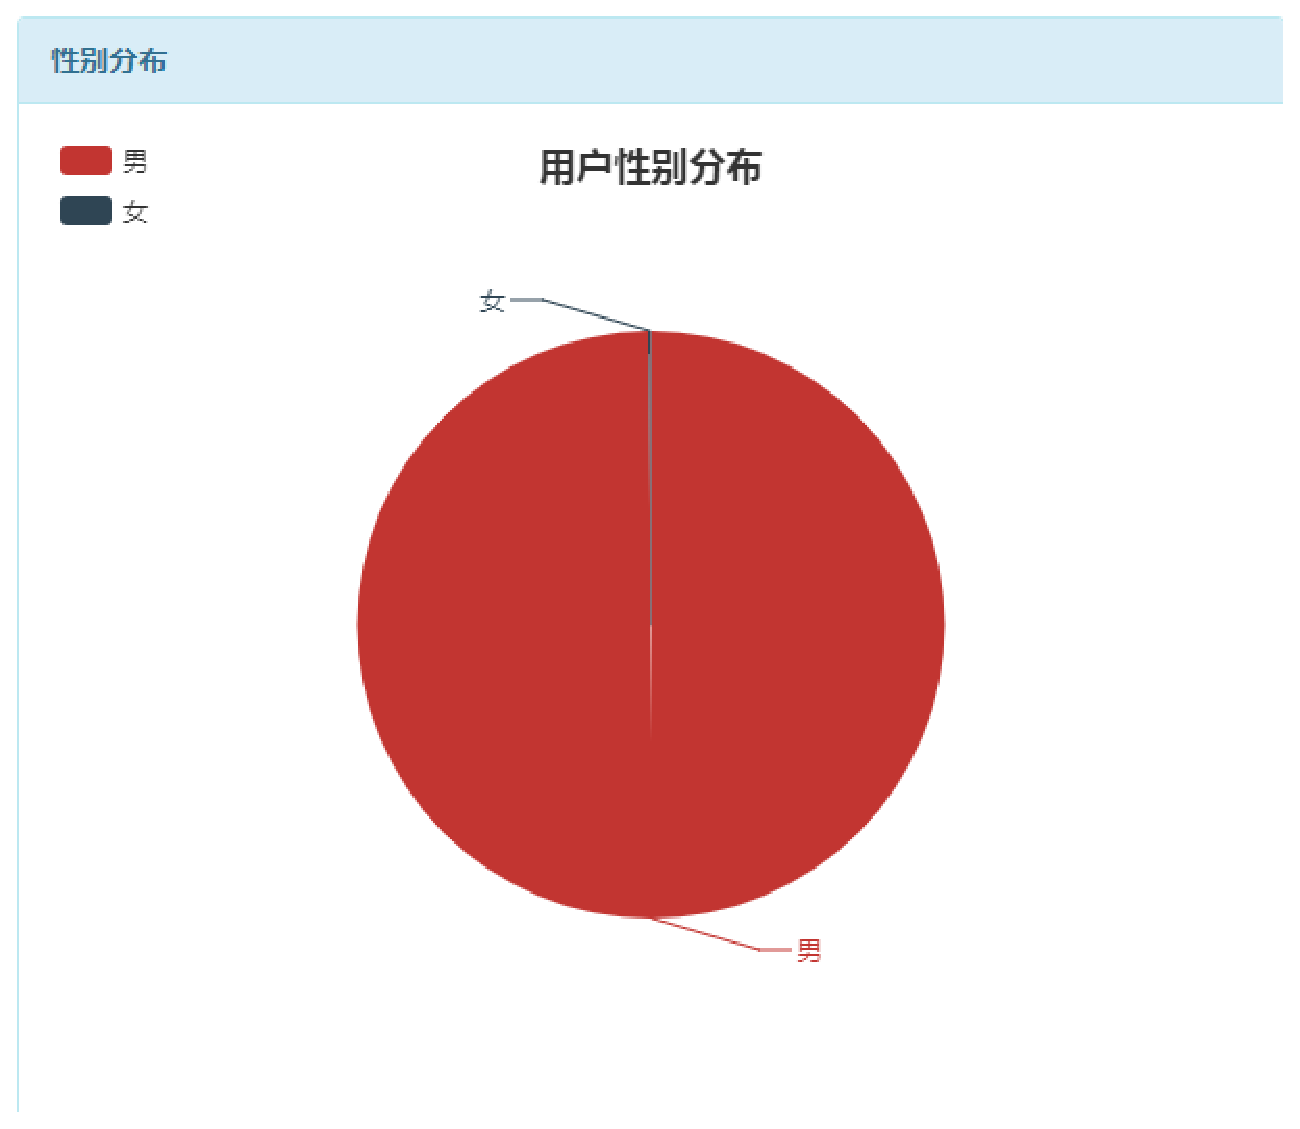
\includegraphics[width=0.15\textwidth]{IMAGE/group-images/11.eps}}
  \subfigure{
      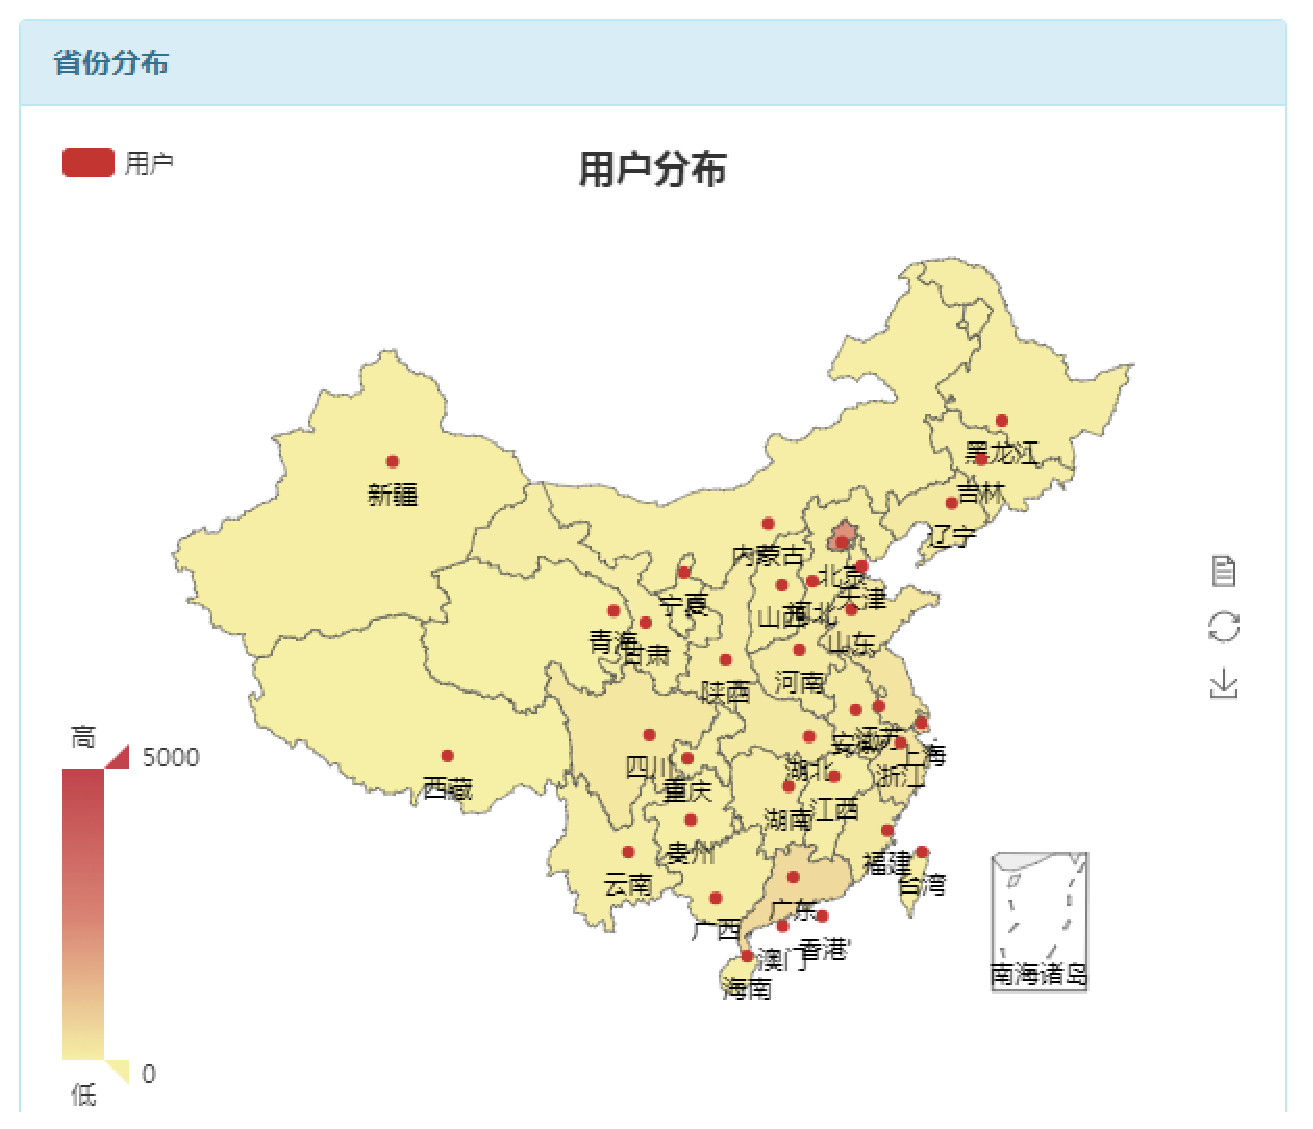
\includegraphics[width=0.15\textwidth]{IMAGE/group-images/12.eps}}
  \subfigure{
      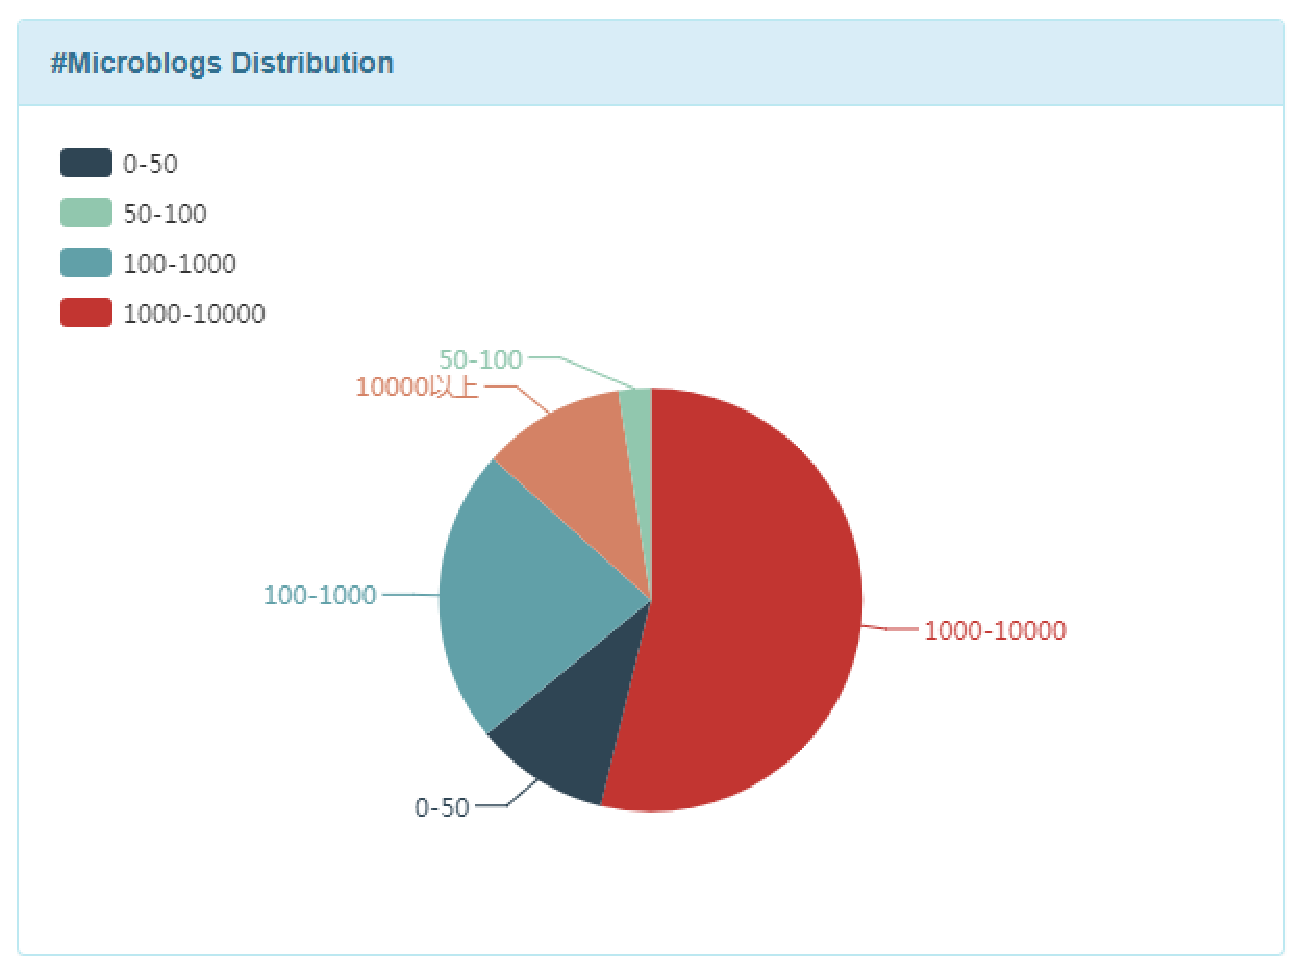
\includegraphics[width=0.15\textwidth]{IMAGE/group-images/13.eps}}
  \subfigure{
      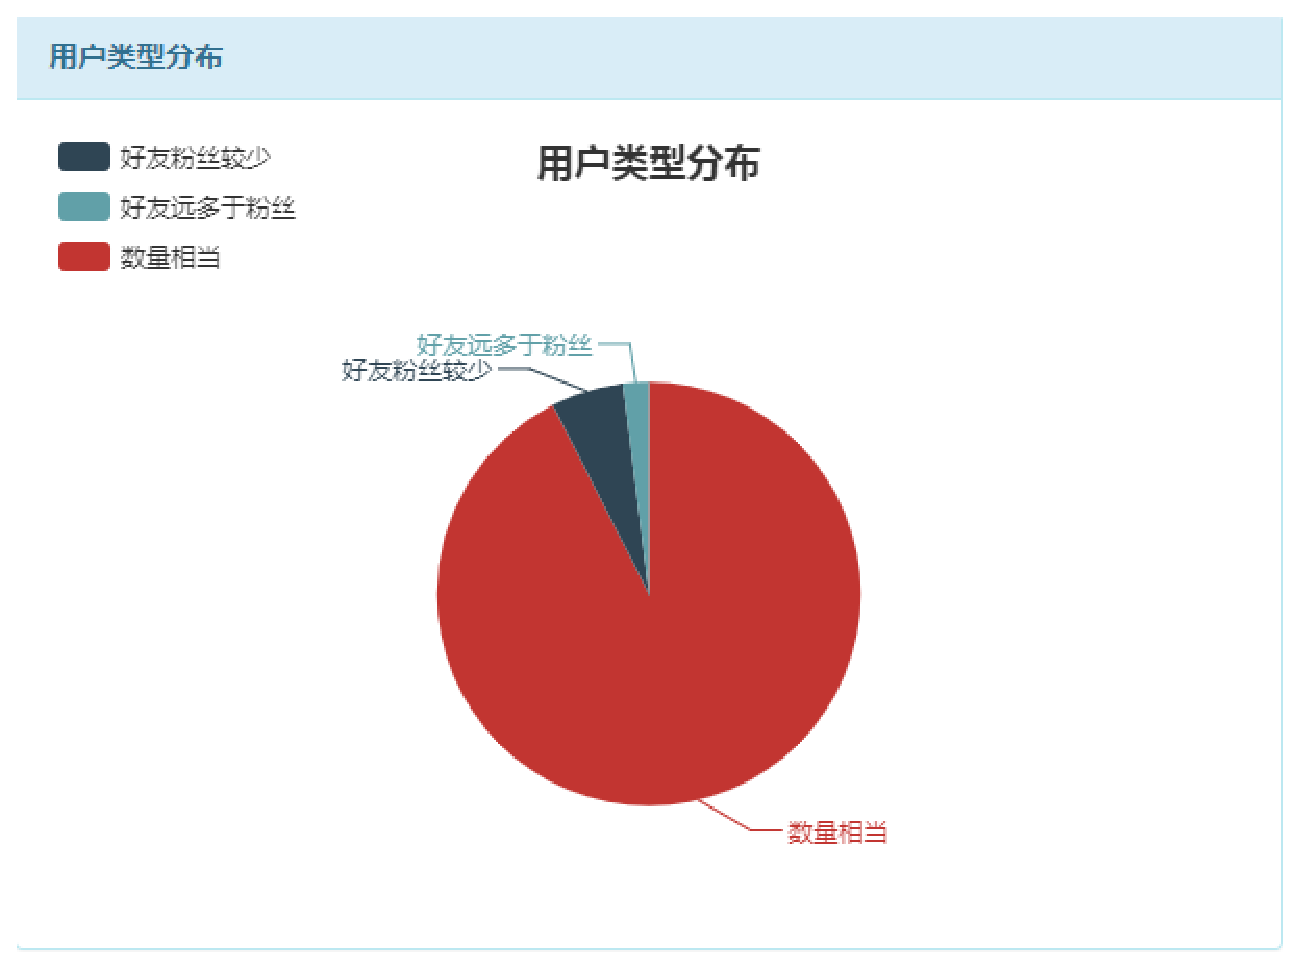
\includegraphics[width=0.15\textwidth]{IMAGE/group-images/14.eps}}
  \subfigure{
      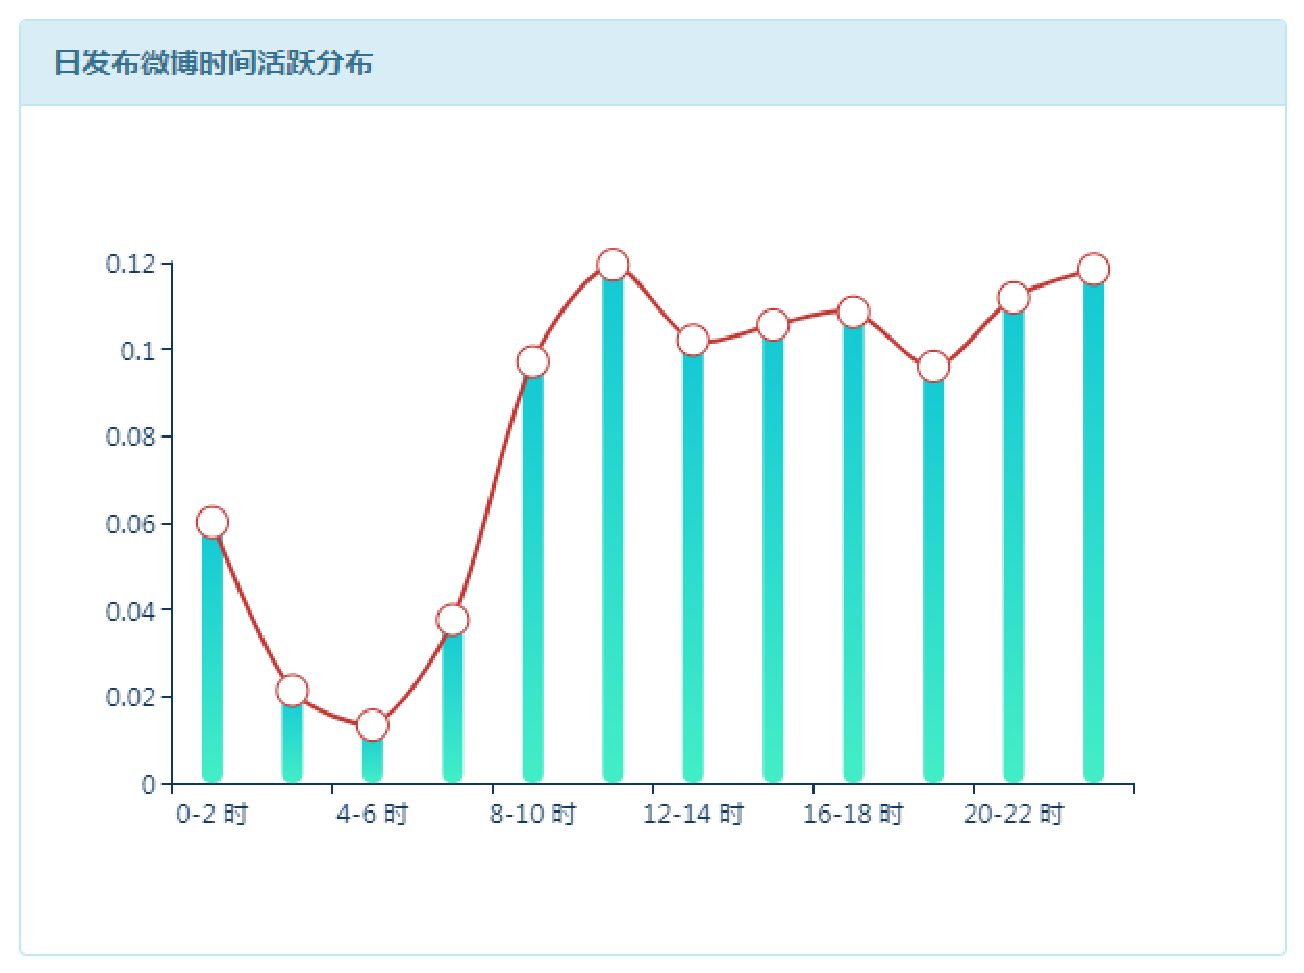
\includegraphics[width=0.15\textwidth]{IMAGE/group-images/15.eps}}
  \subfigure{
      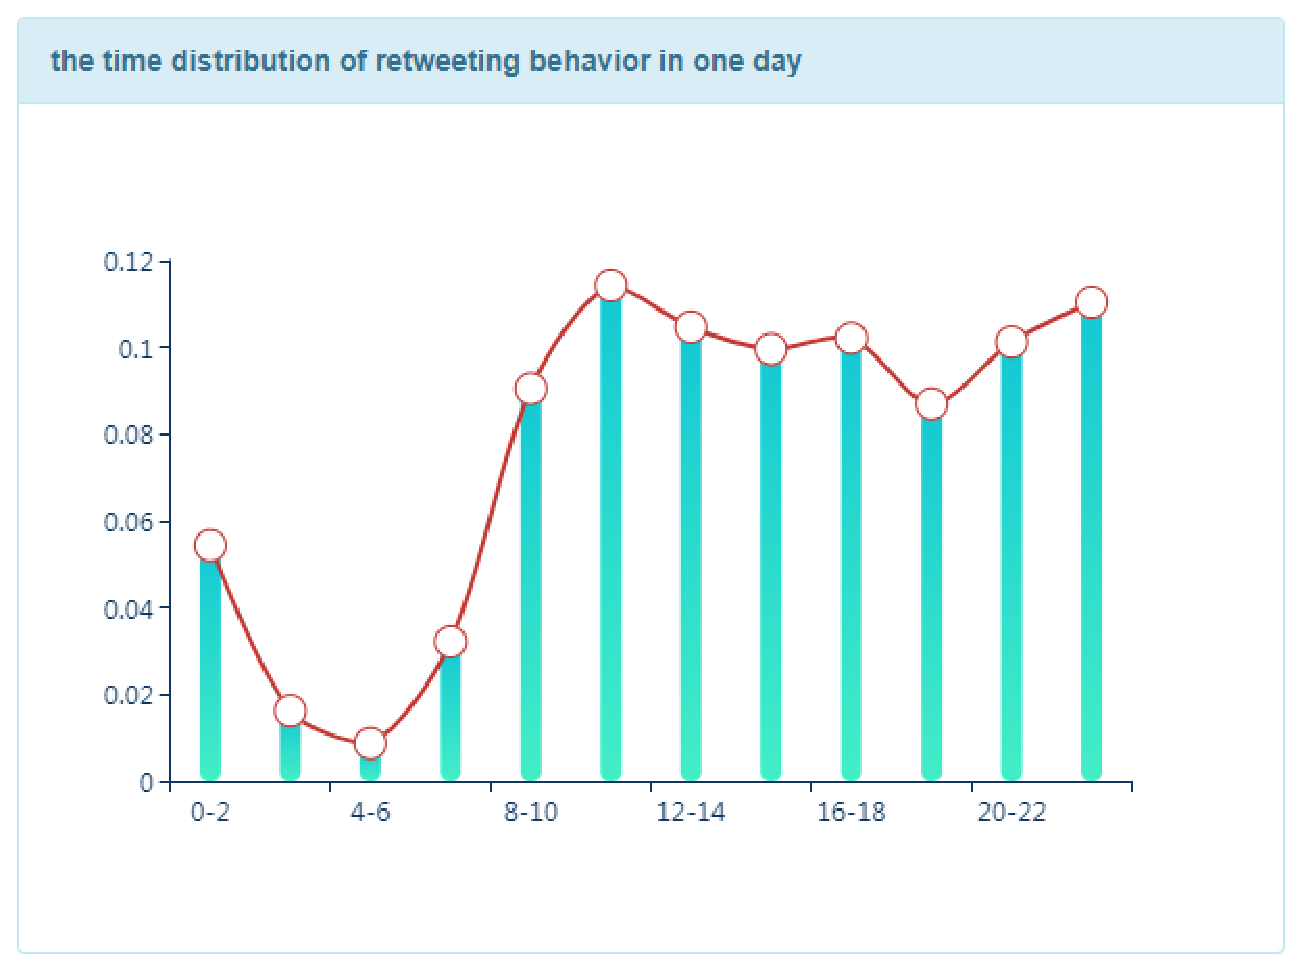
\includegraphics[width=0.15\textwidth]{IMAGE/group-images/16.eps}}
  \subfigure{
      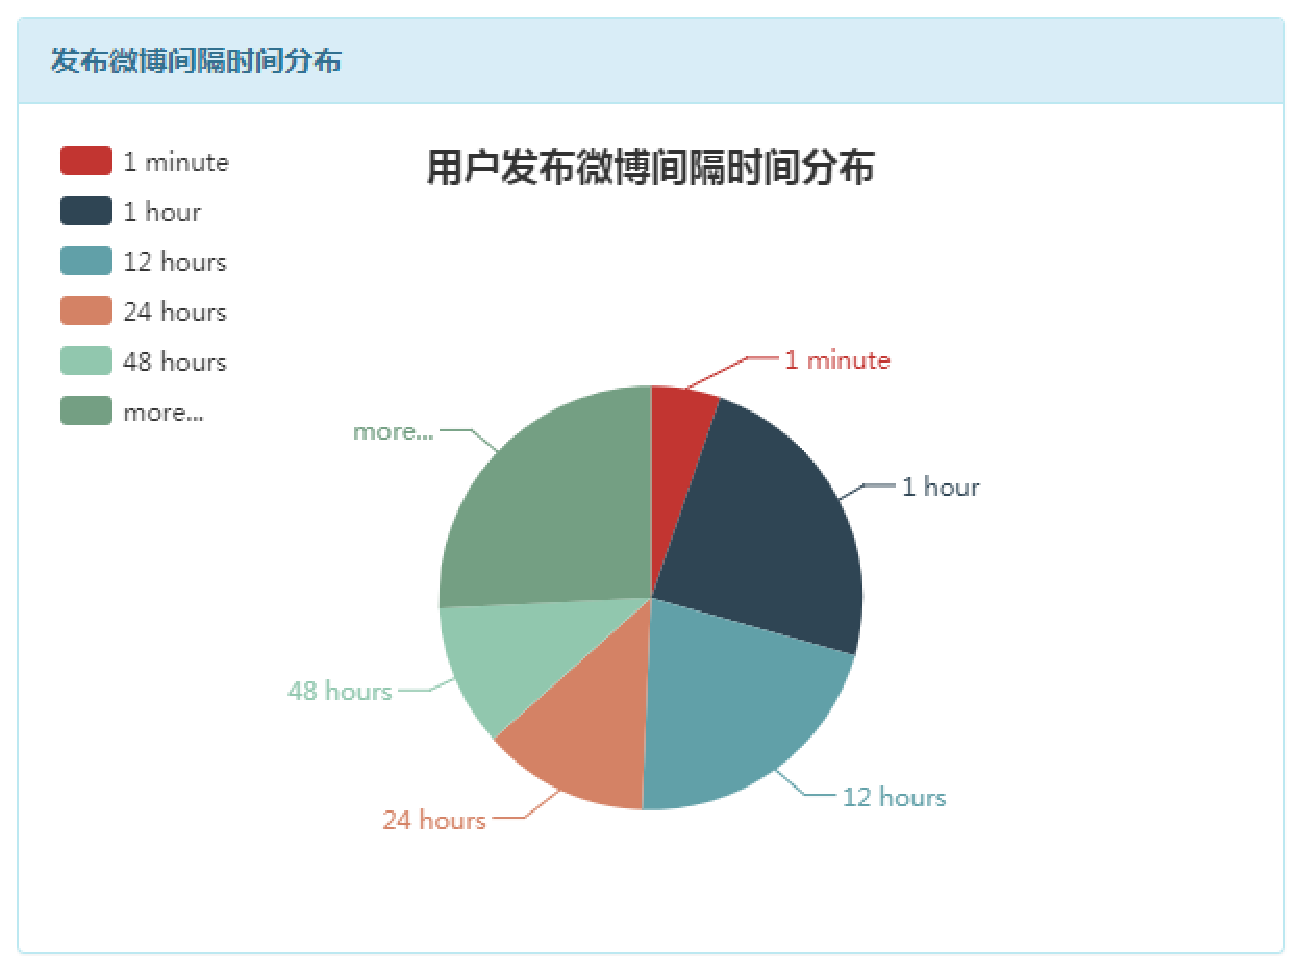
\includegraphics[width=0.15\textwidth]{IMAGE/group-images/17.eps}}
  \subfigure{
      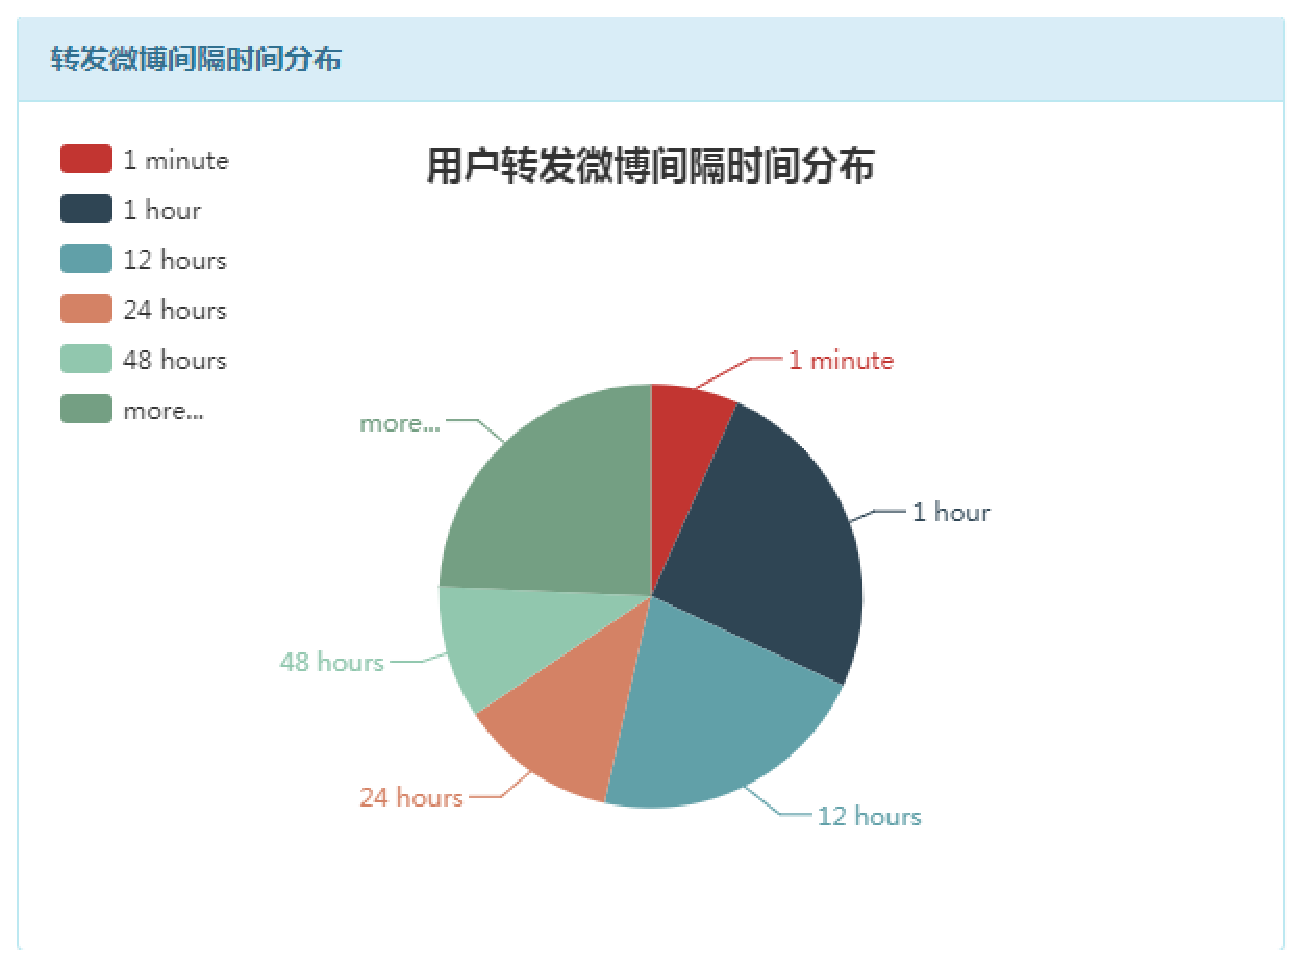
\includegraphics[width=0.15\textwidth]{IMAGE/group-images/18.eps}}
  \subfigure{
      
\includegraphics[width=0.15\textwidth]{IMAGE/group-images/19.eps}}
  \caption{The Statistics of User Group One}
  \label{fig:subfig} %% label for entire figure
\end{figure}
\begin{figure}
  \centering
  \subfigure{
      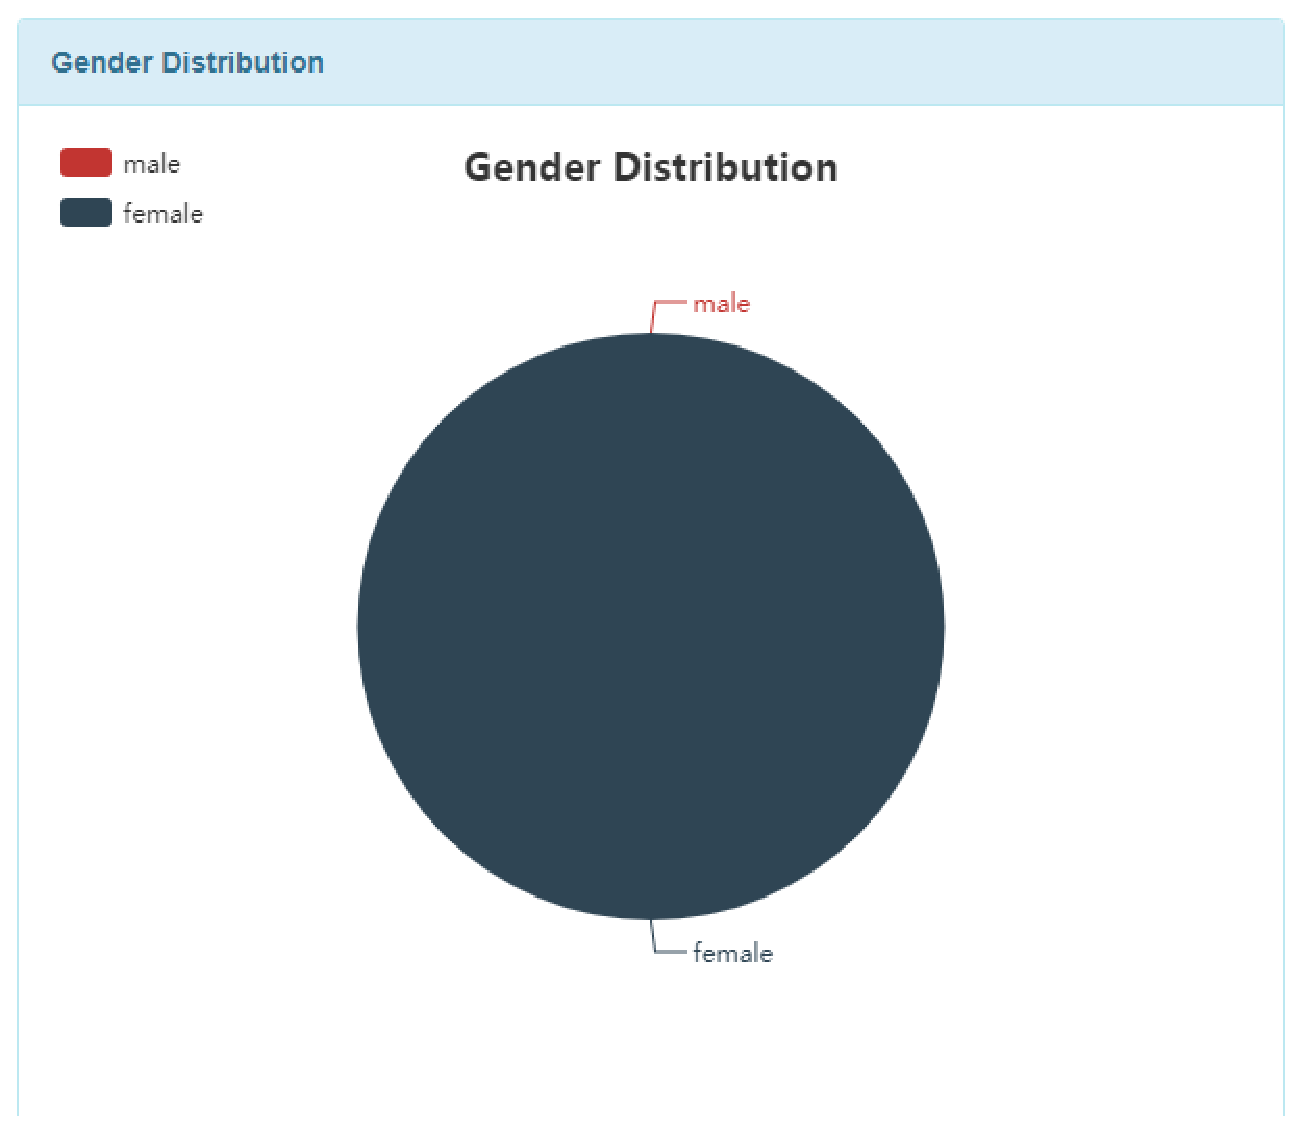
\includegraphics[width=0.15\textwidth]{IMAGE/group-images/21.eps}}
  \subfigure{
      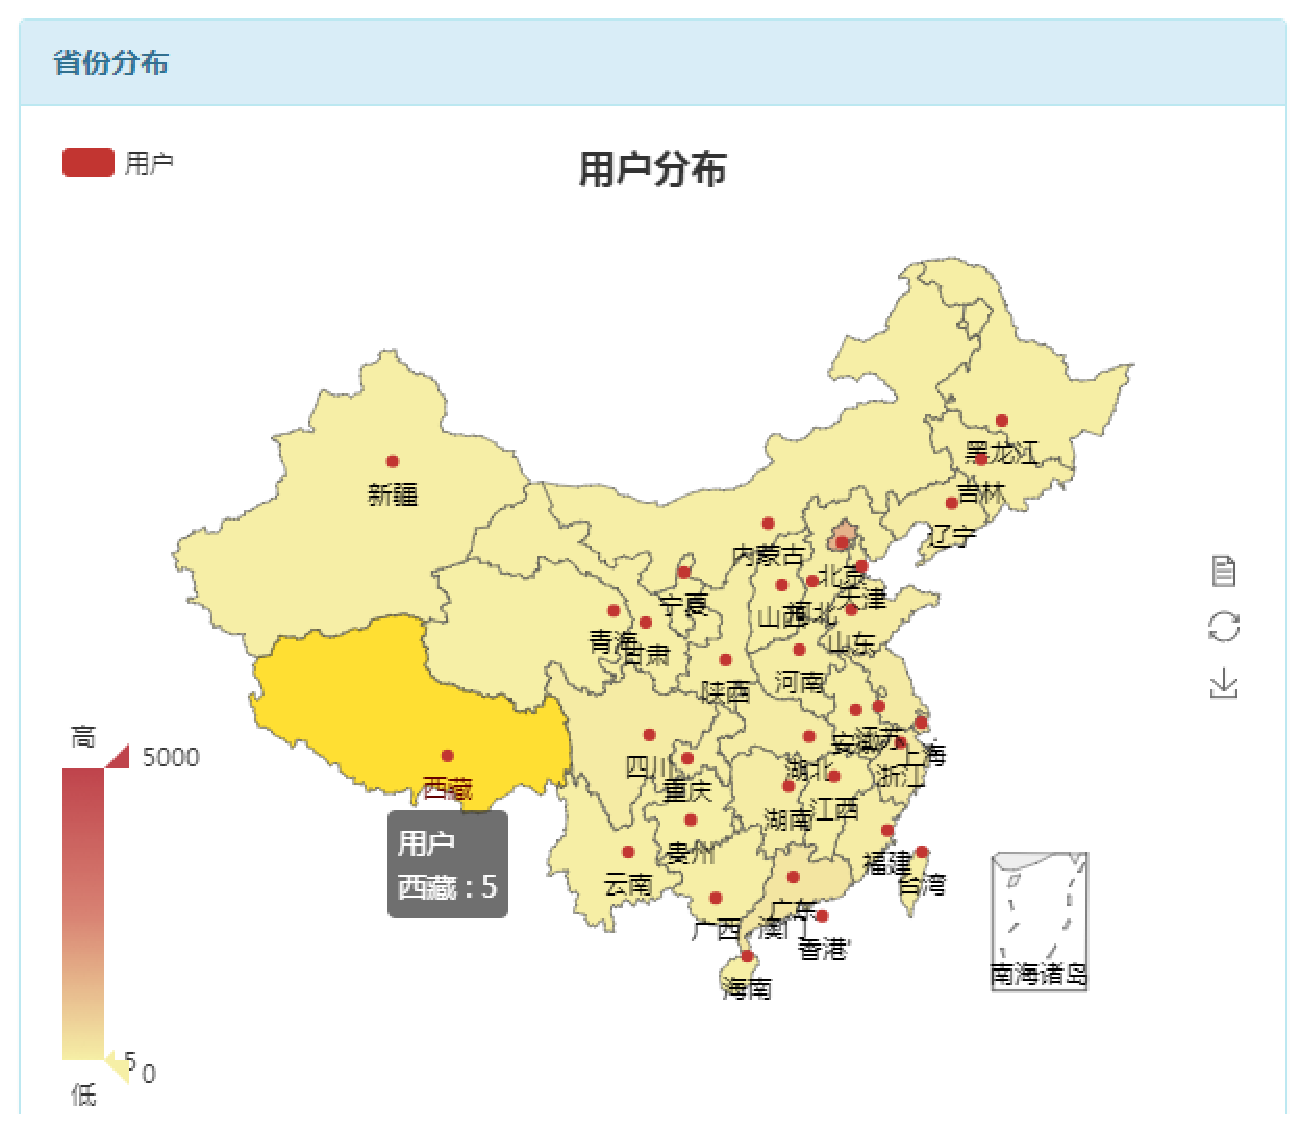
\includegraphics[width=0.15\textwidth]{IMAGE/group-images/22.eps}}
  \subfigure{
      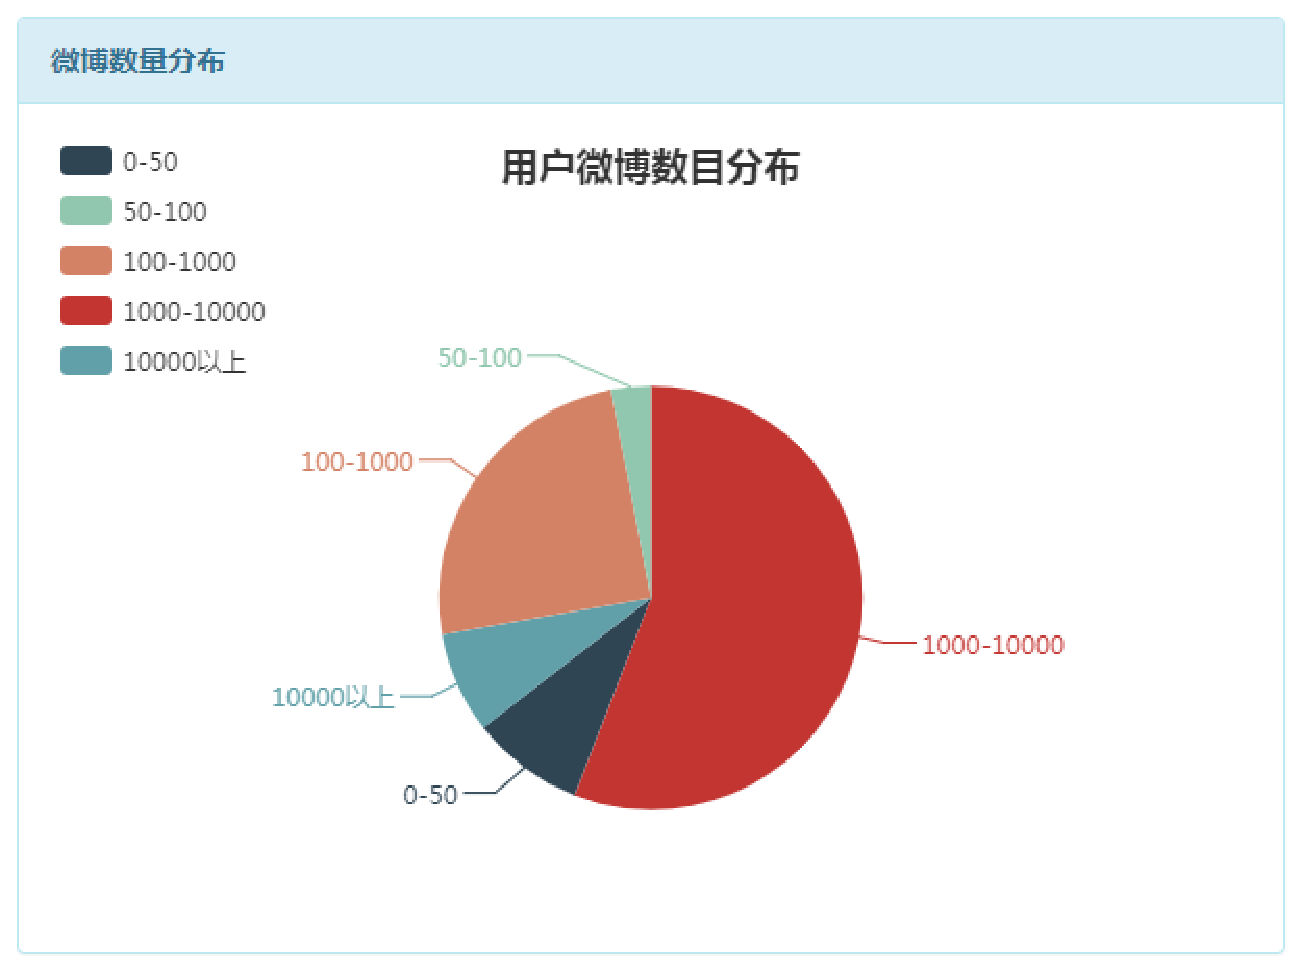
\includegraphics[width=0.15\textwidth]{IMAGE/group-images/23.eps}}
  \subfigure{
      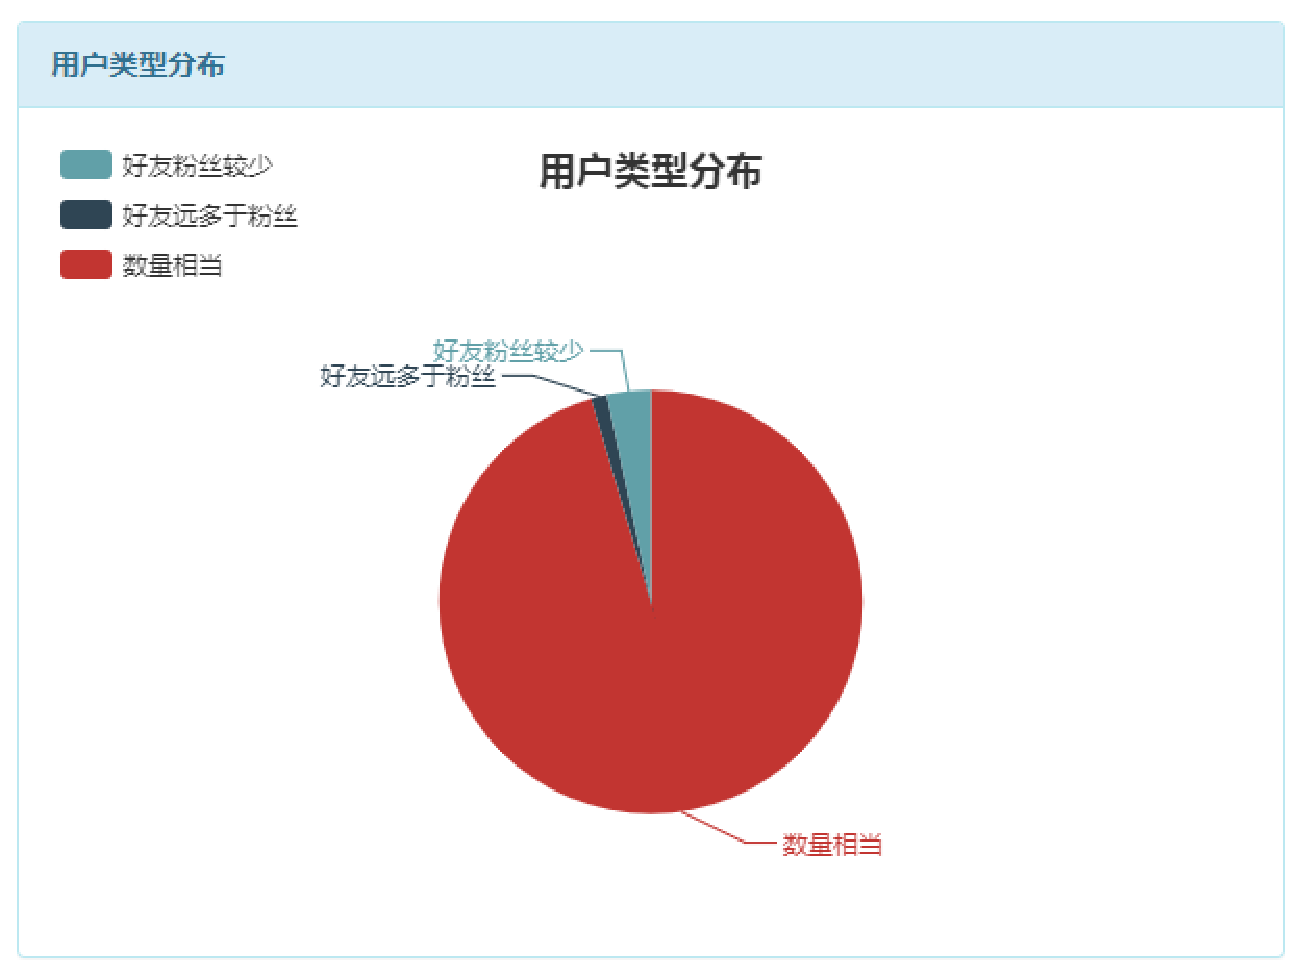
\includegraphics[width=0.15\textwidth]{IMAGE/group-images/24.eps}}
  \subfigure{
      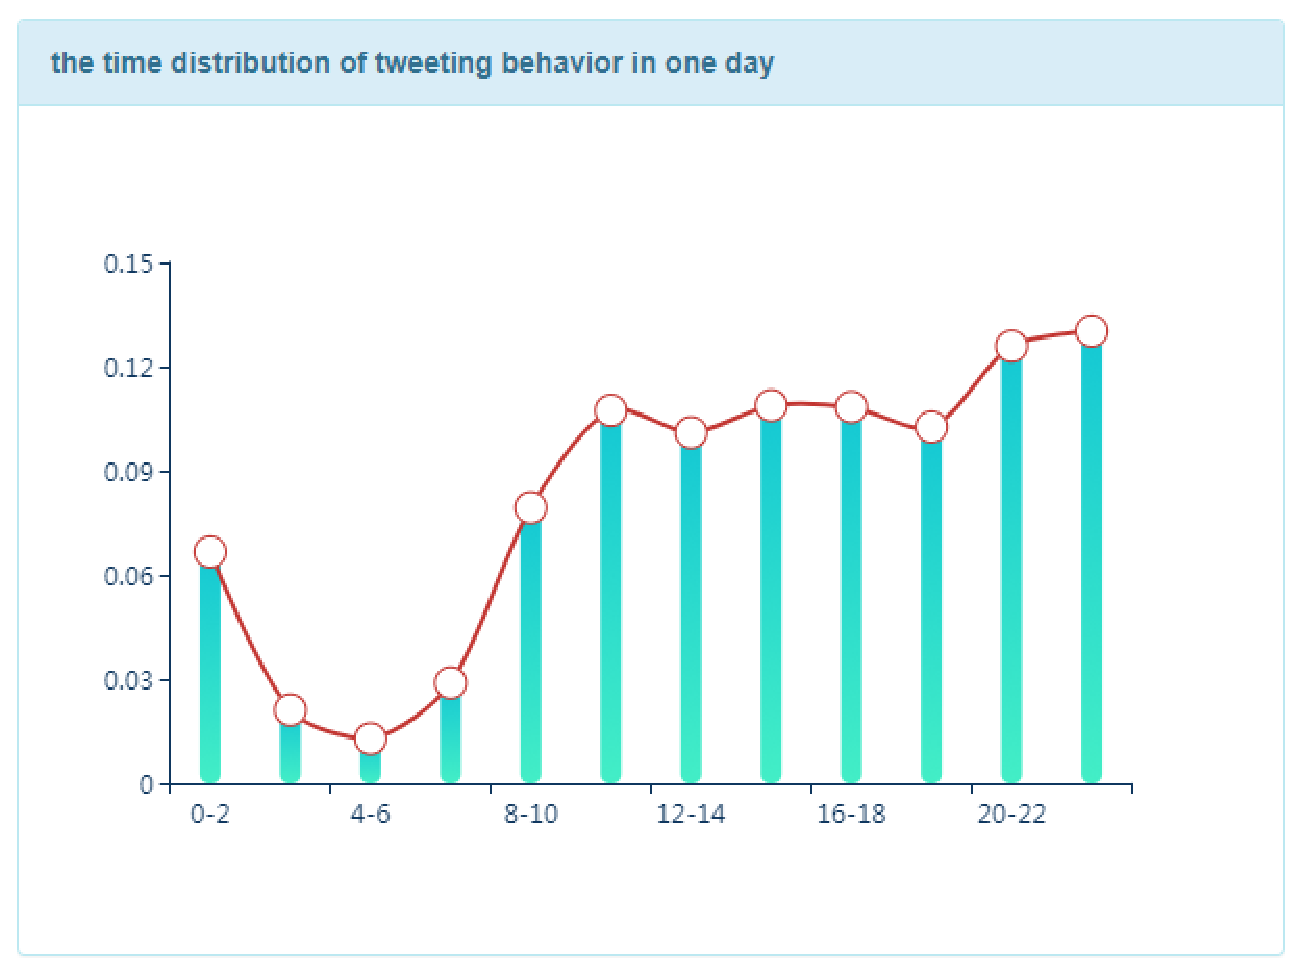
\includegraphics[width=0.15\textwidth]{IMAGE/group-images/25.eps}}
  \subfigure{
      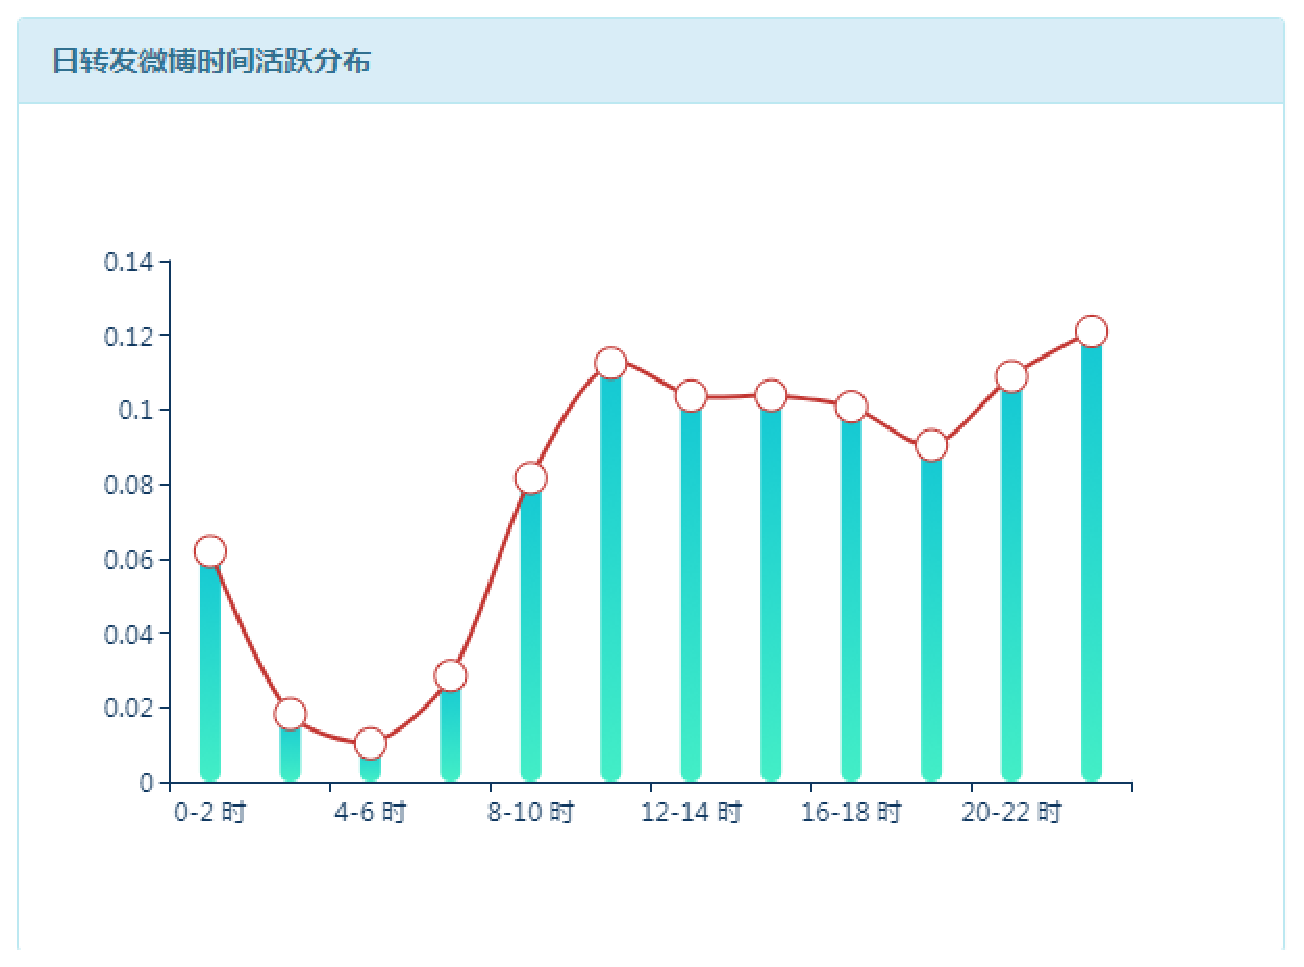
\includegraphics[width=0.15\textwidth]{IMAGE/group-images/26.eps}}
  \subfigure{
      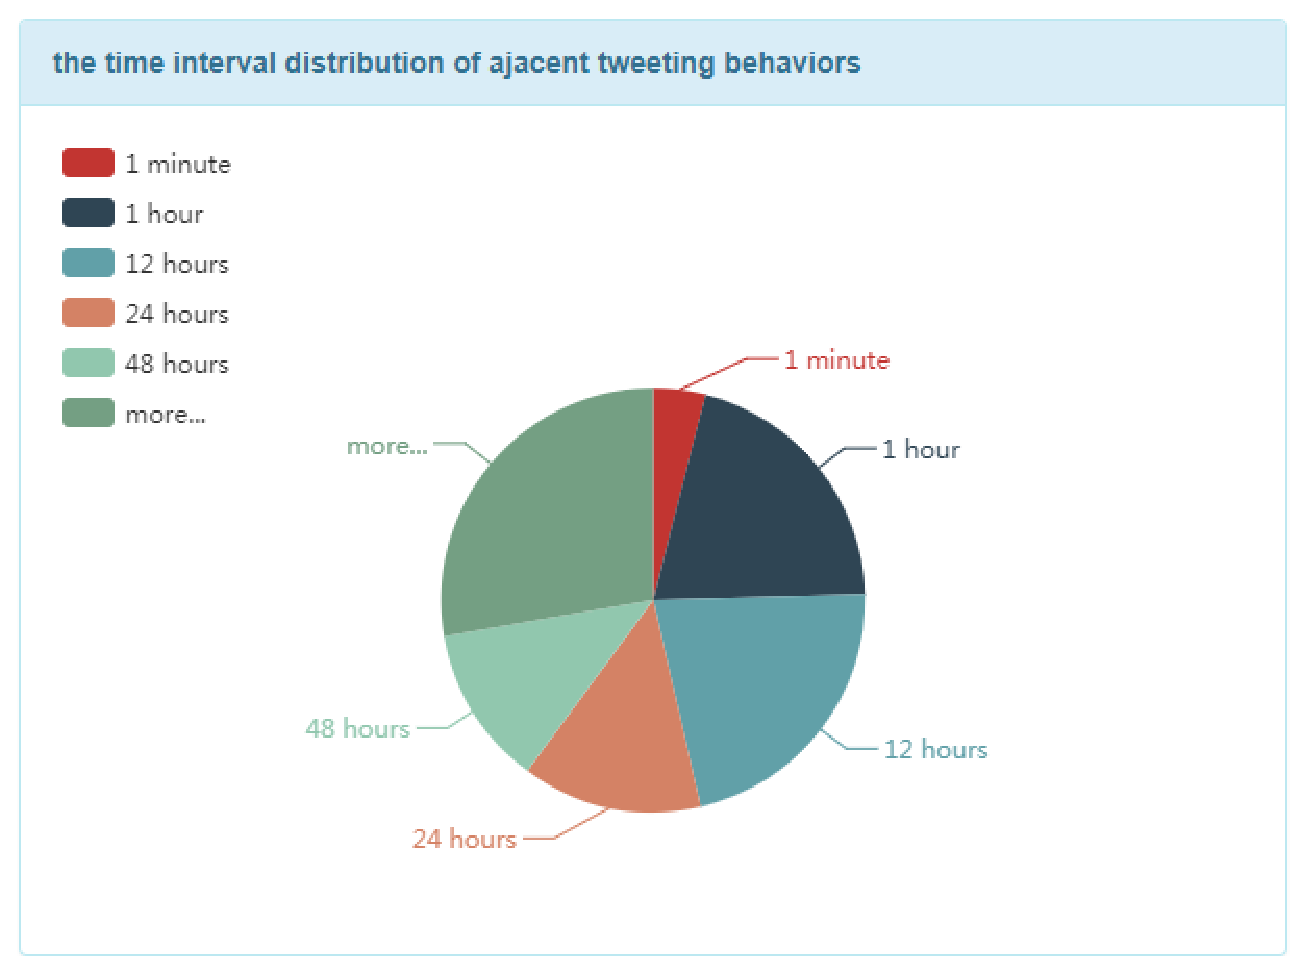
\includegraphics[width=0.15\textwidth]{IMAGE/group-images/27.eps}}
  \subfigure{
      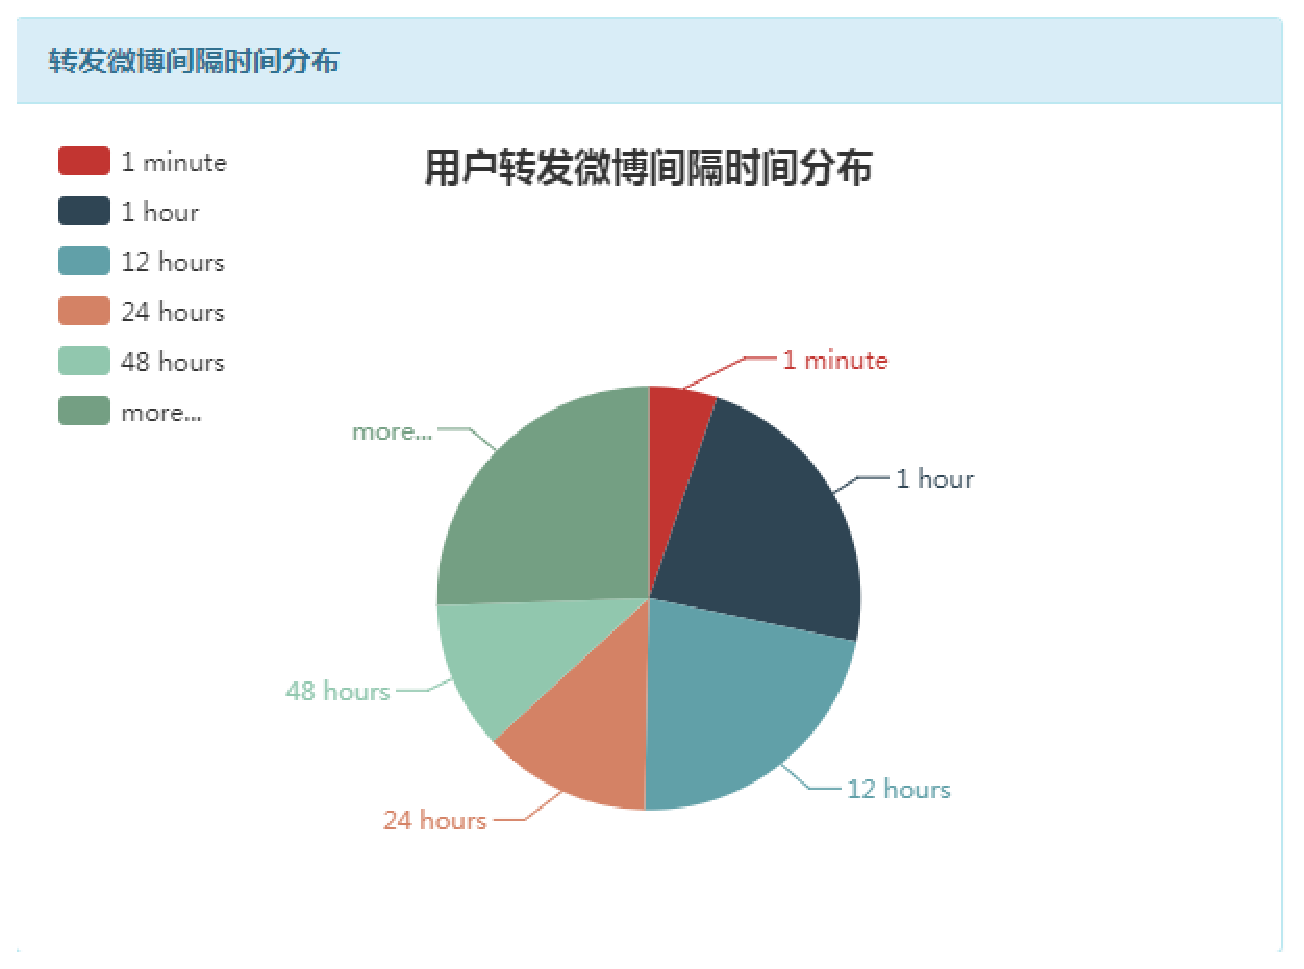
\includegraphics[width=0.15\textwidth]{IMAGE/group-images/28.eps}}
  \subfigure{
      
\includegraphics[width=0.15\textwidth]{IMAGE/group-images/29.eps}}
  \caption{The Statistics of User Group Two}
  \label{fig:subfig} %% label for entire figure
\end{figure}
\begin{figure}
  \centering
  \subfigure{
      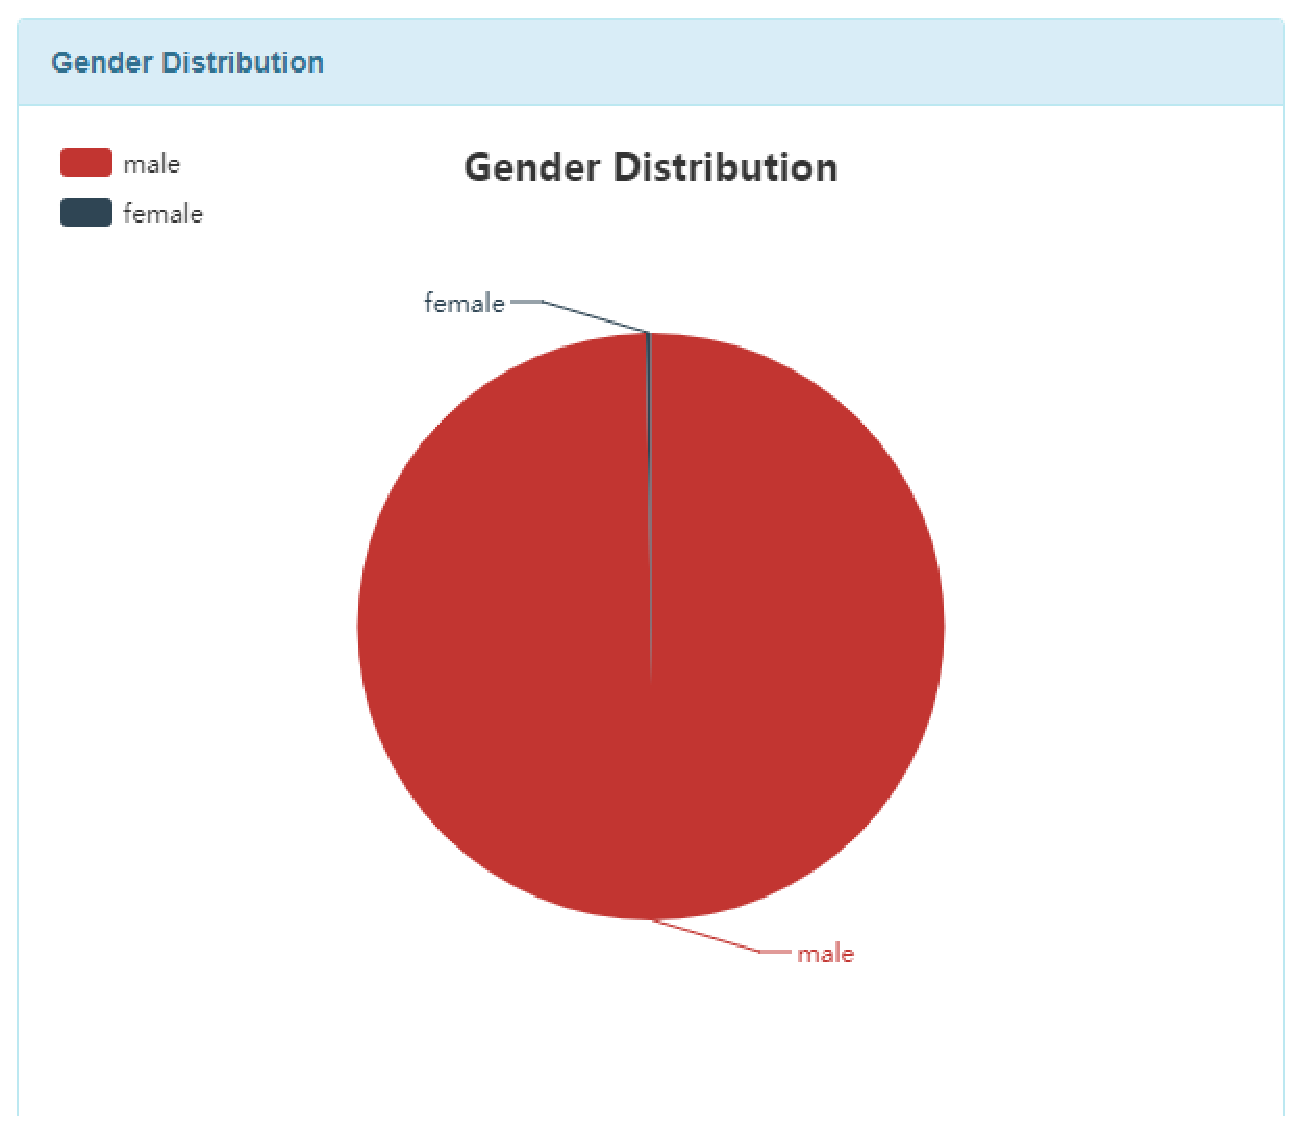
\includegraphics[width=0.15\textwidth]{IMAGE/group-images/31.eps}}
  \subfigure{
      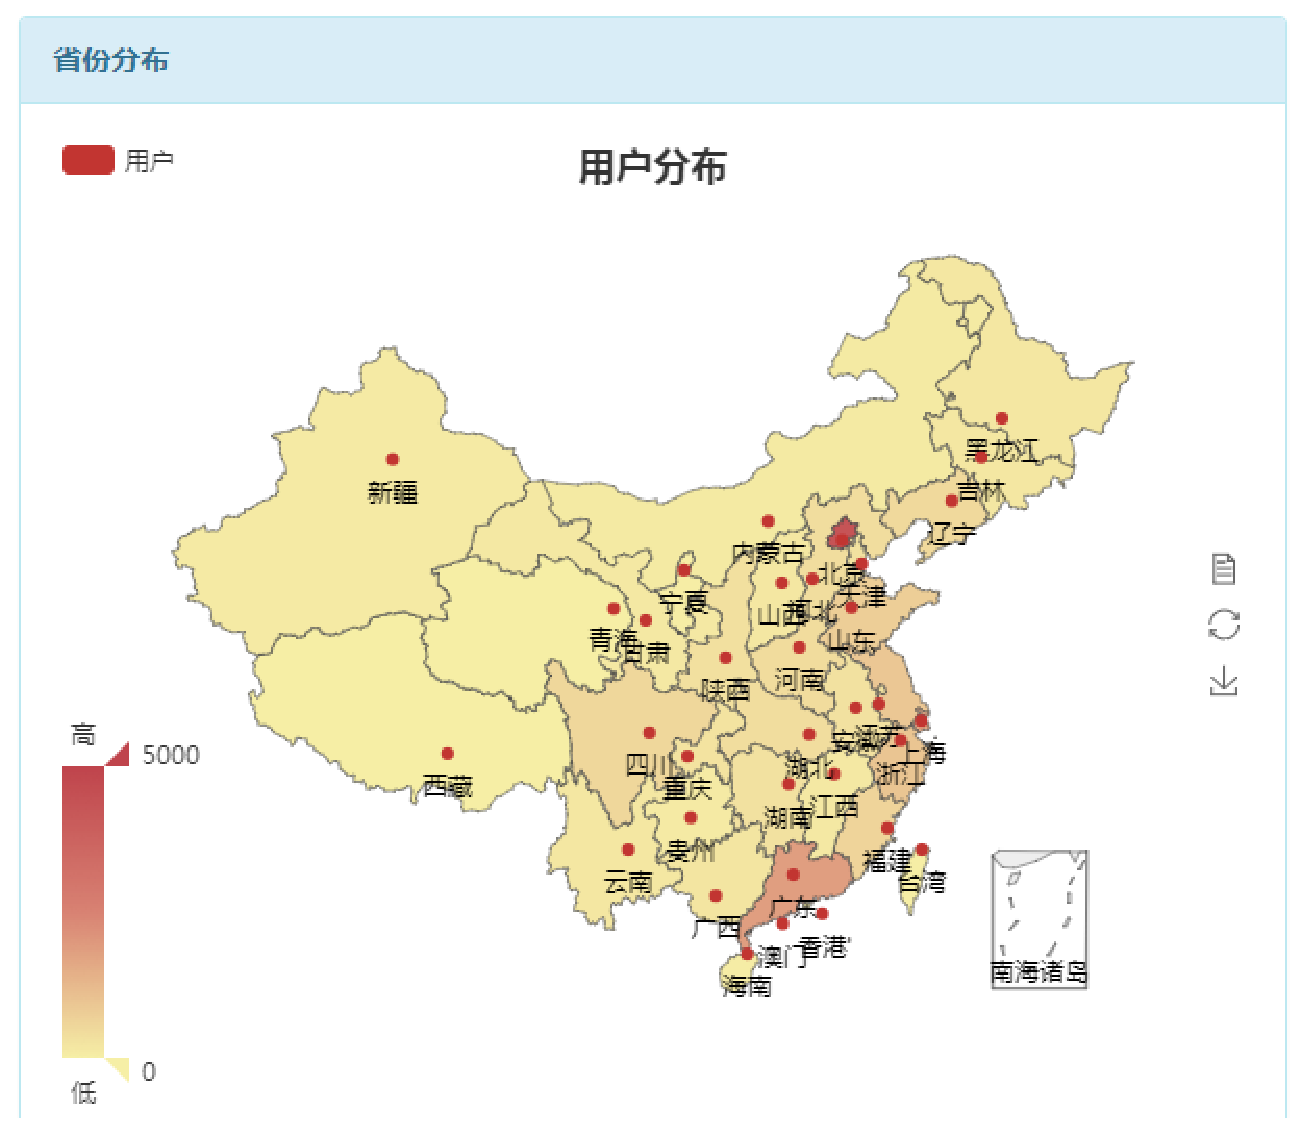
\includegraphics[width=0.15\textwidth]{IMAGE/group-images/32.eps}}
  \subfigure{
      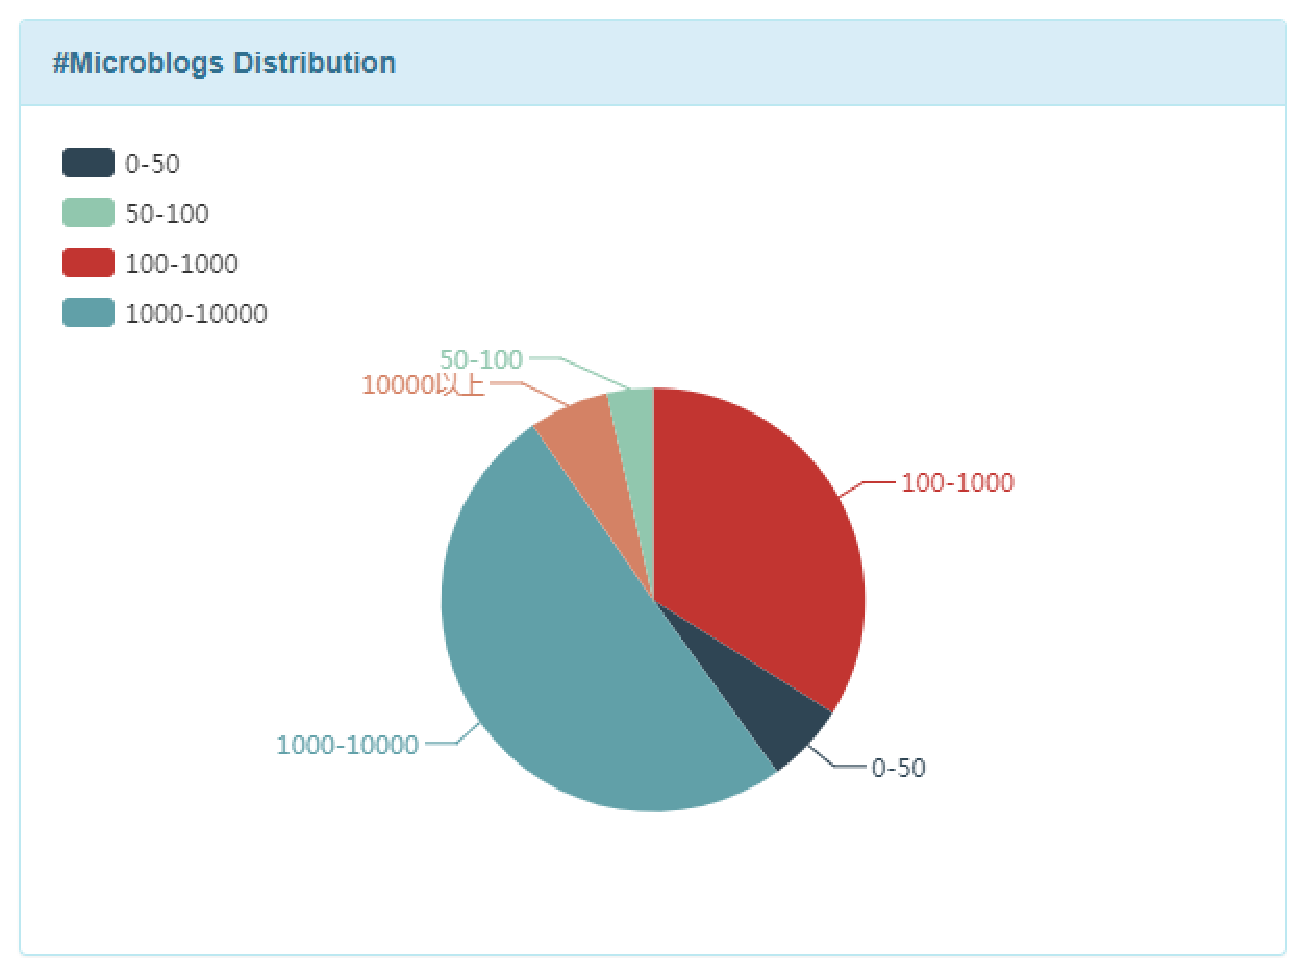
\includegraphics[width=0.15\textwidth]{IMAGE/group-images/33.eps}}
  \subfigure{
      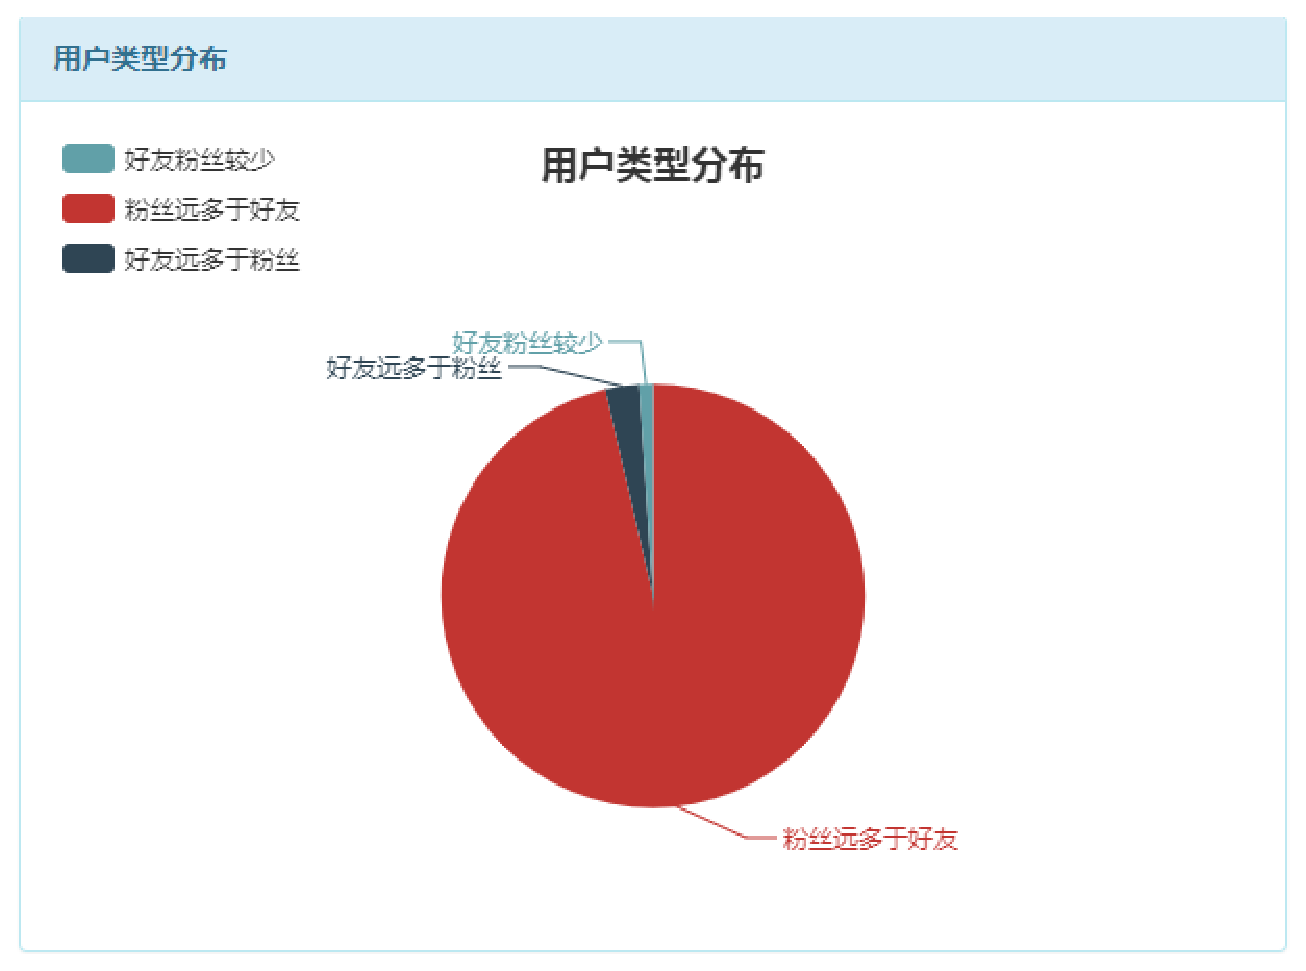
\includegraphics[width=0.15\textwidth]{IMAGE/group-images/34.eps}}
  \subfigure{
      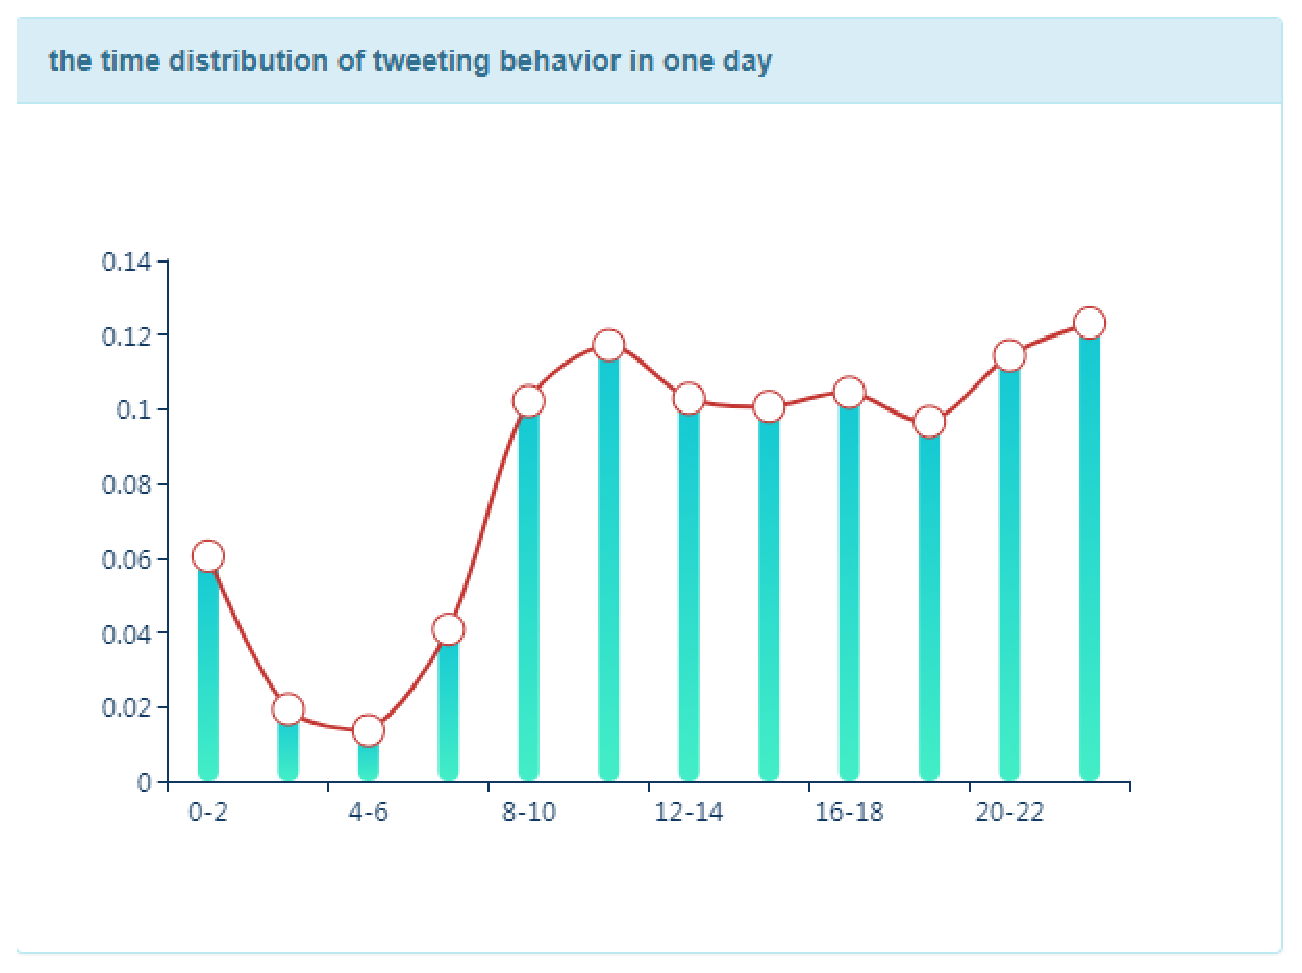
\includegraphics[width=0.15\textwidth]{IMAGE/group-images/35.eps}}
  \subfigure{
      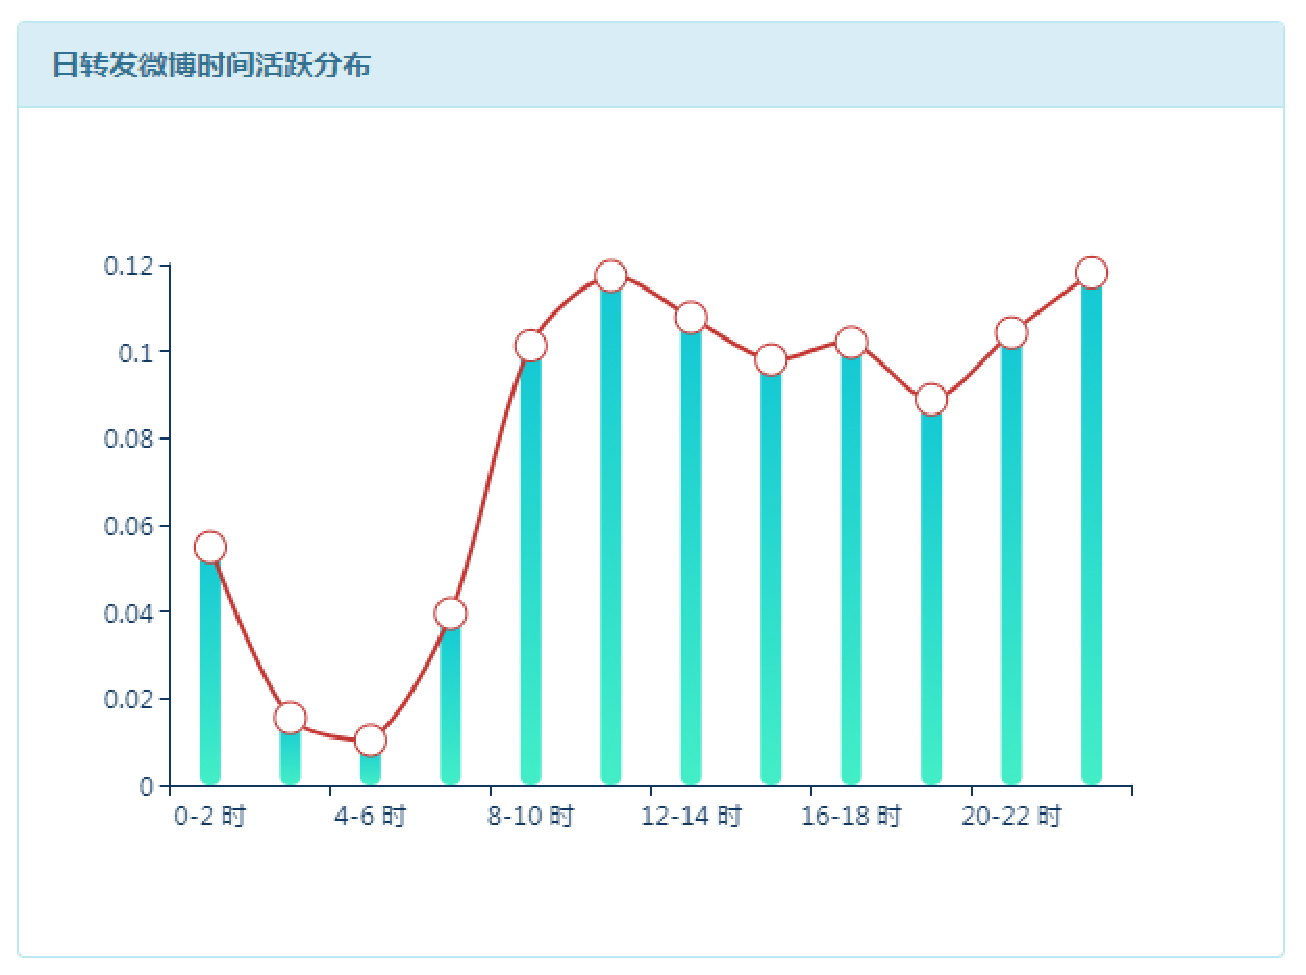
\includegraphics[width=0.15\textwidth]{IMAGE/group-images/36.eps}}
  \subfigure{
      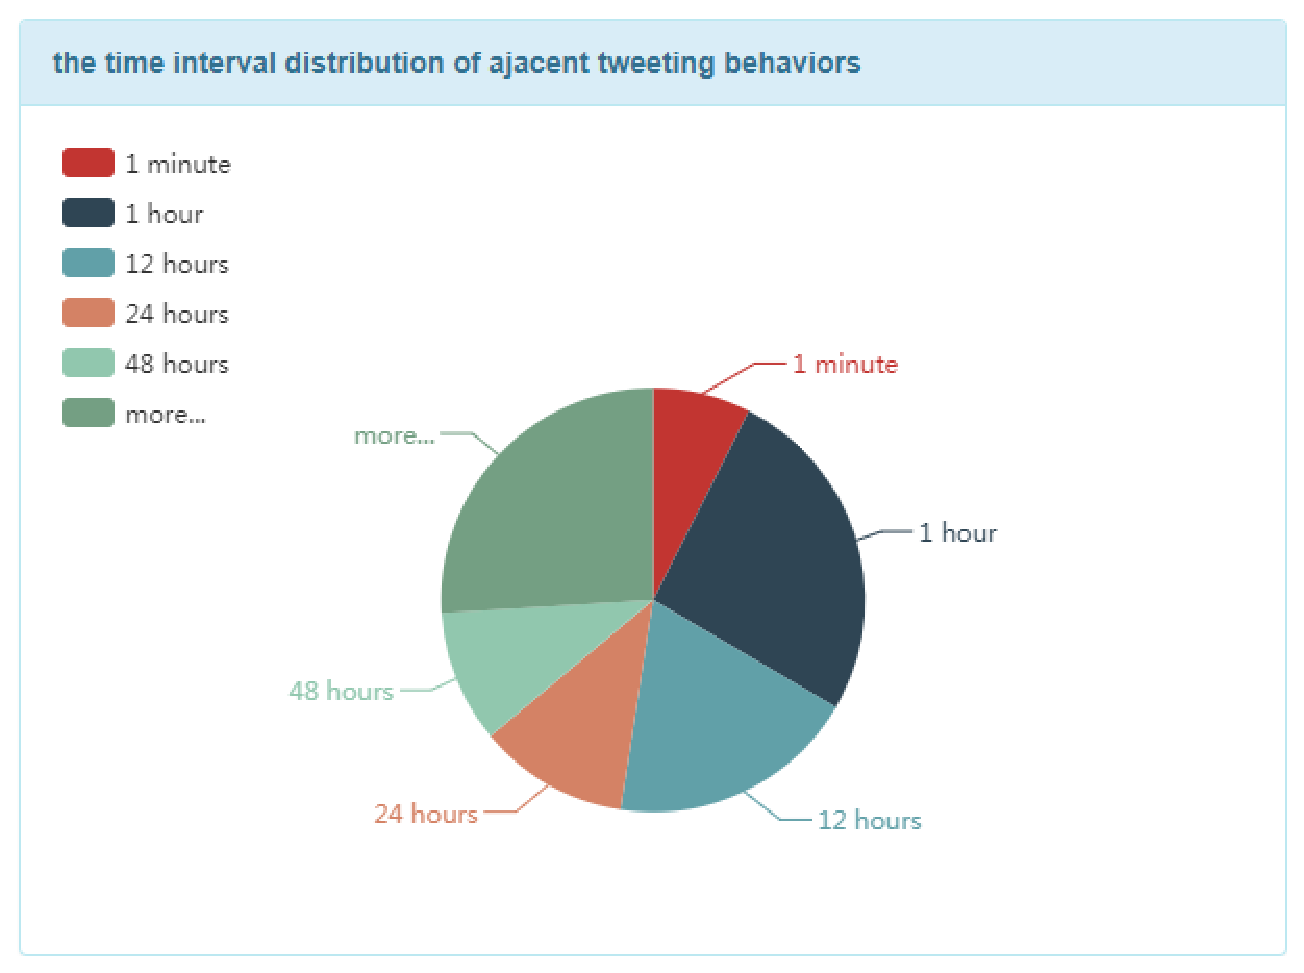
\includegraphics[width=0.15\textwidth]{IMAGE/group-images/37.eps}}
  \subfigure{
      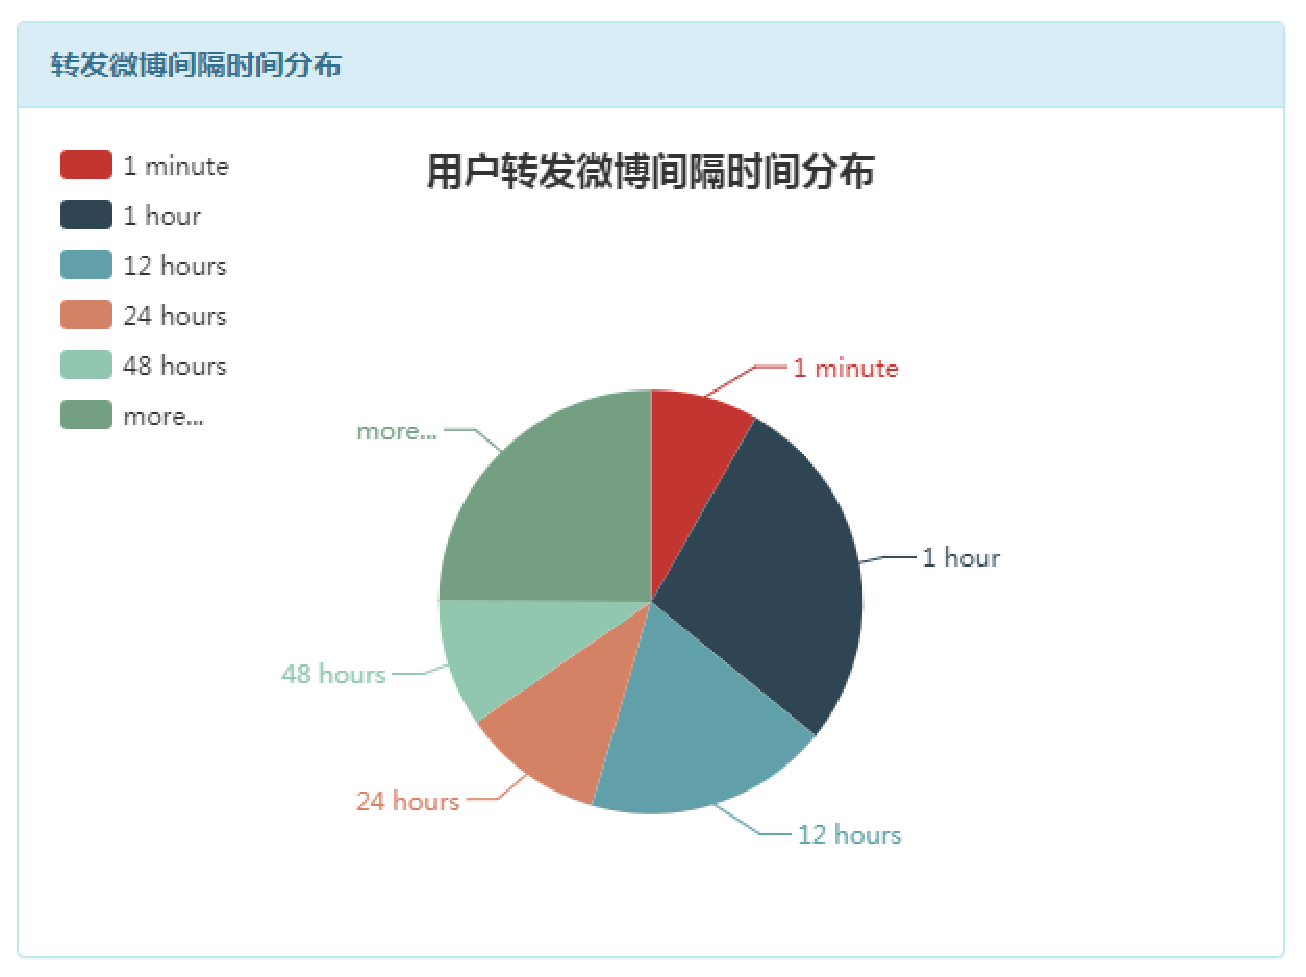
\includegraphics[width=0.15\textwidth]{IMAGE/group-images/38.eps}}
  \subfigure{
      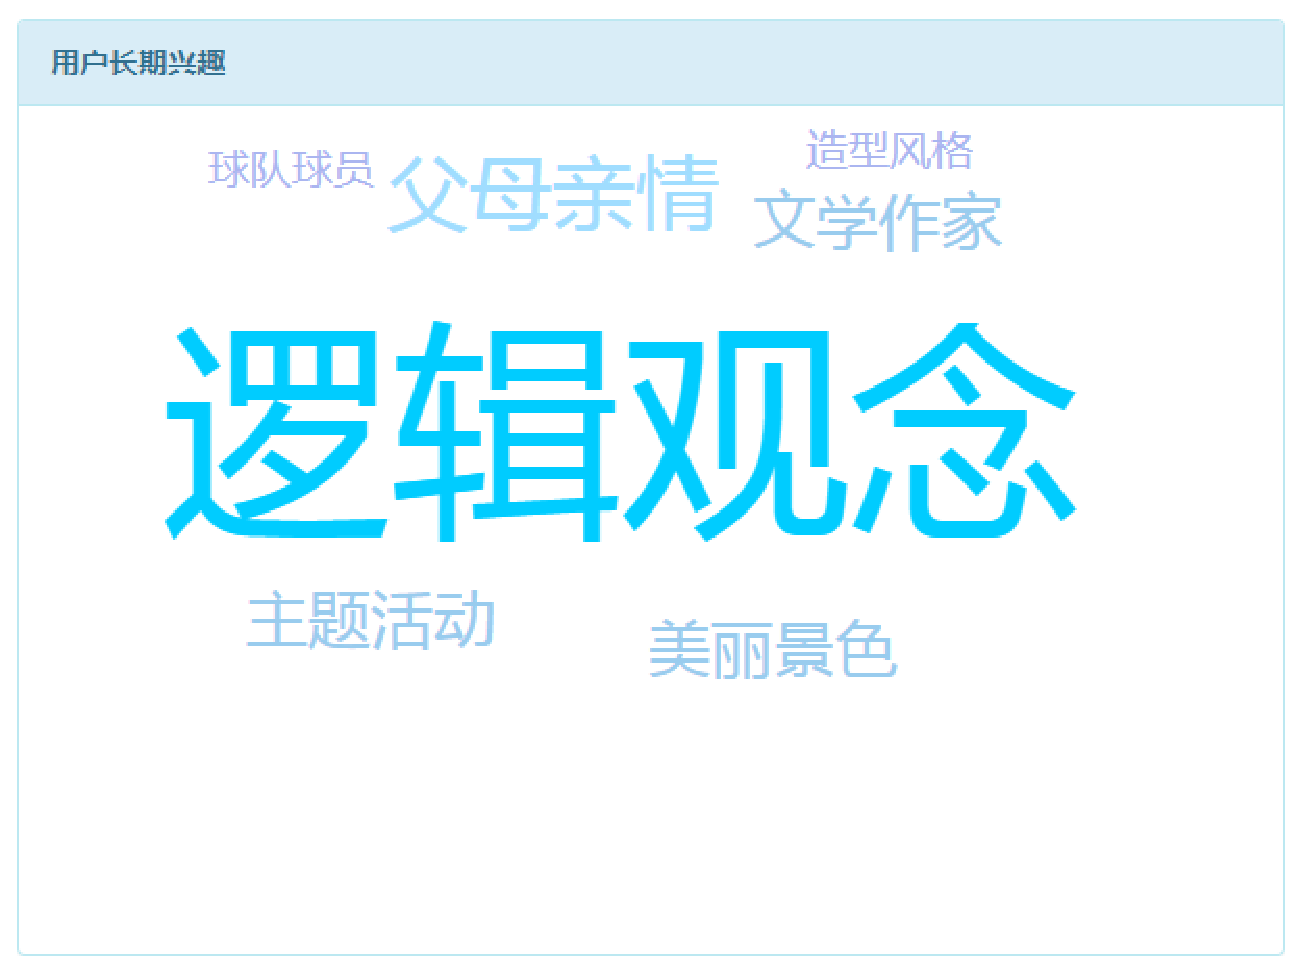
\includegraphics[width=0.15\textwidth]{IMAGE/group-images/39.eps}}
  \caption{The Statistics of User Group Three}
  \label{fig:subfig} %% label for entire figure
\end{figure}
\begin{figure}
  \centering
  \subfigure{
      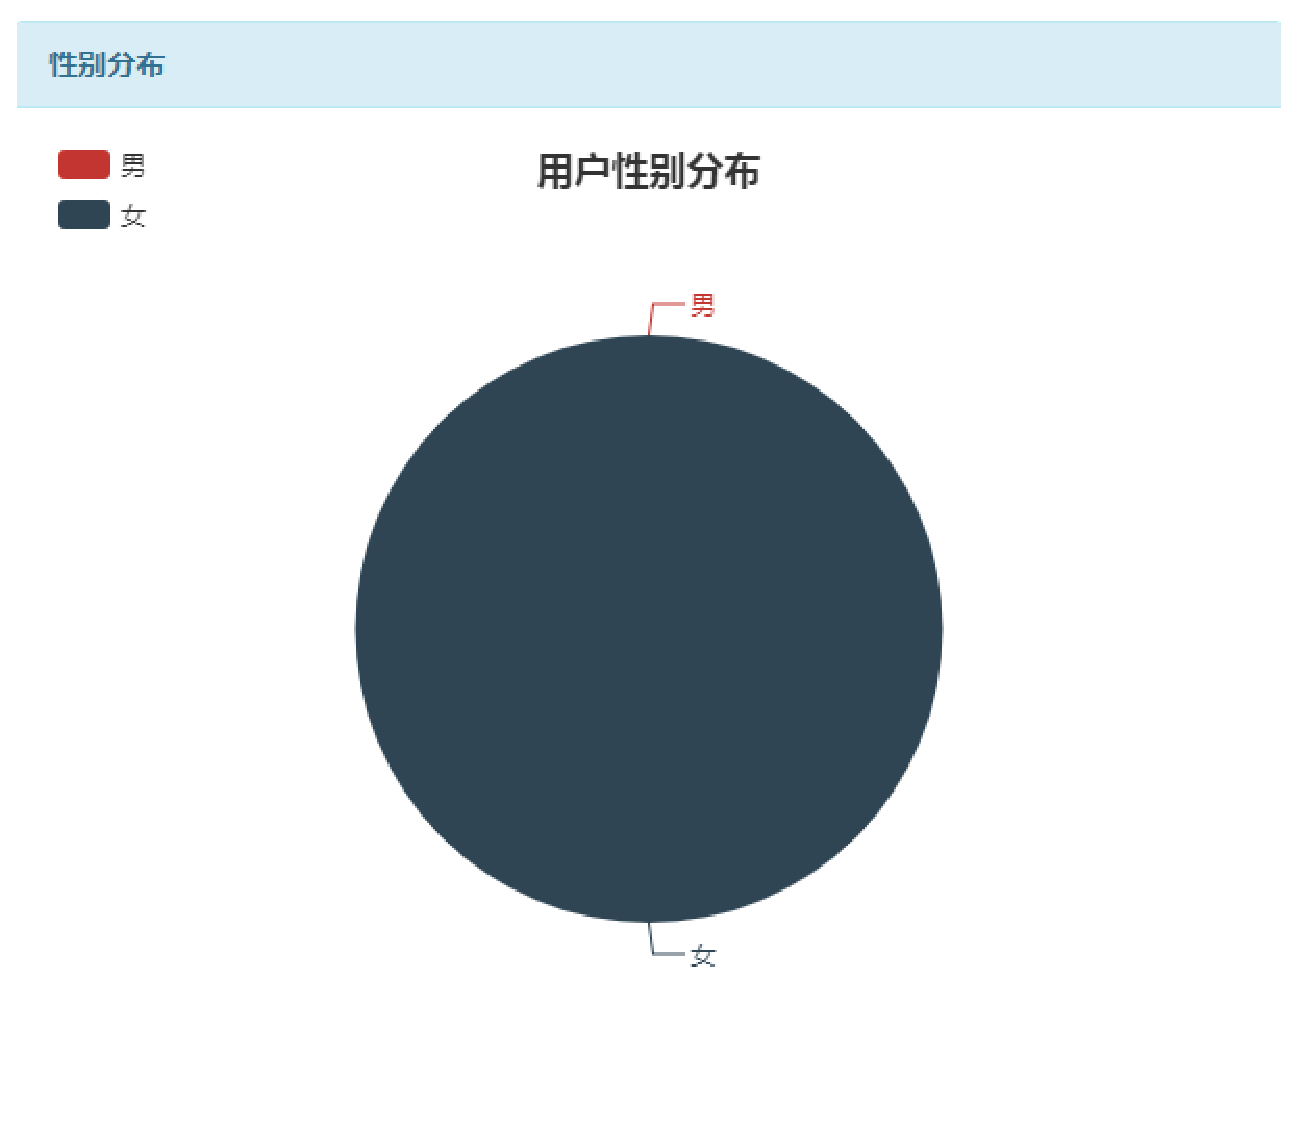
\includegraphics[width=0.15\textwidth]{IMAGE/group-images/41.eps}}
  \subfigure{
      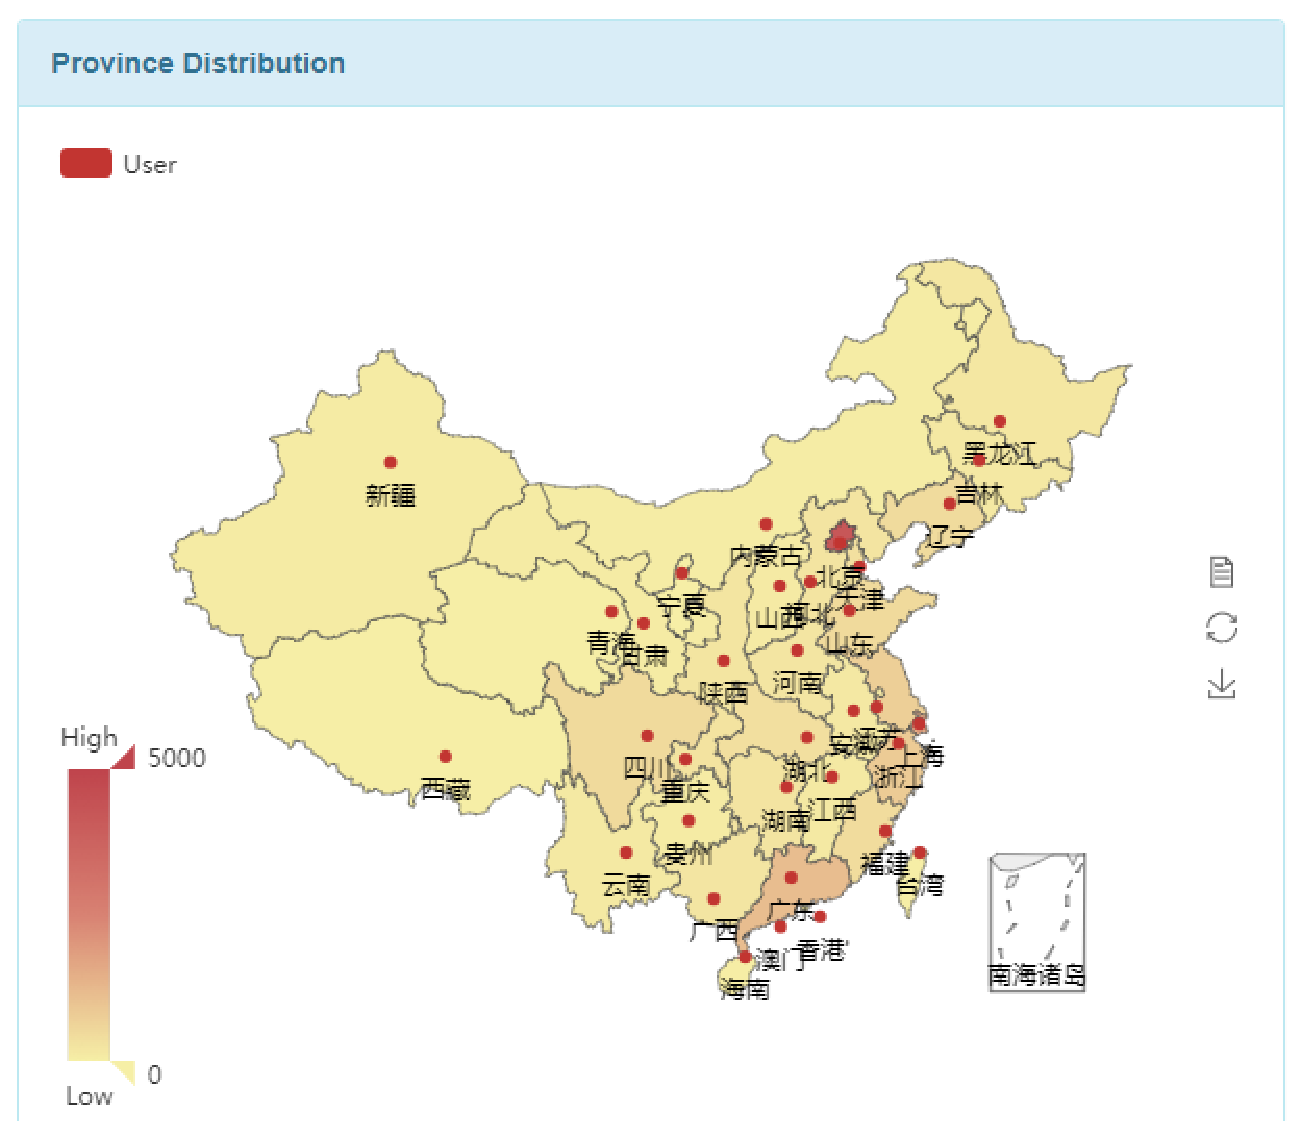
\includegraphics[width=0.15\textwidth]{IMAGE/group-images/42.eps}}
  \subfigure{
      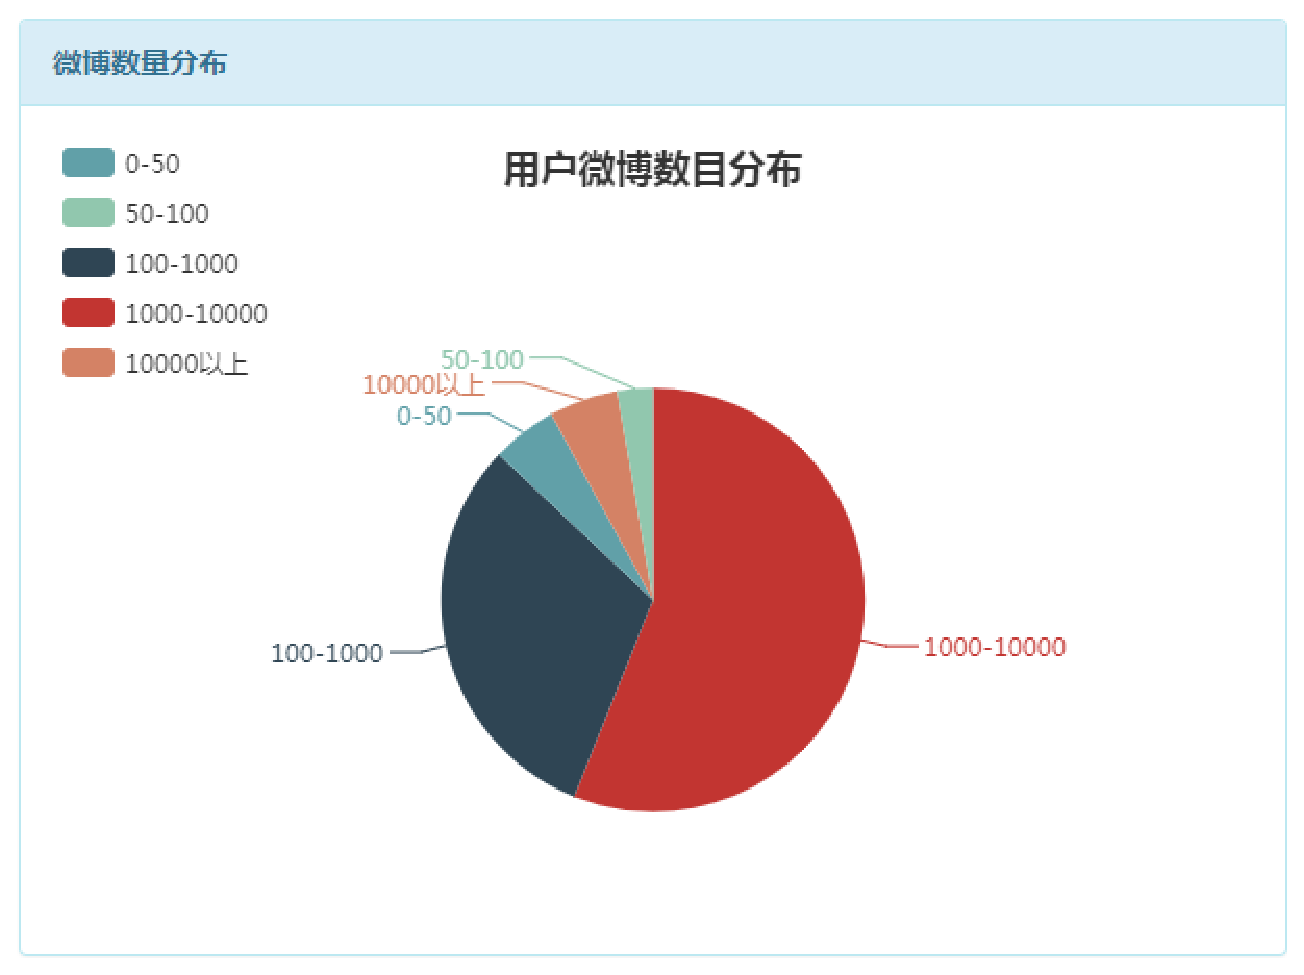
\includegraphics[width=0.15\textwidth]{IMAGE/group-images/43.eps}}
  \subfigure{
      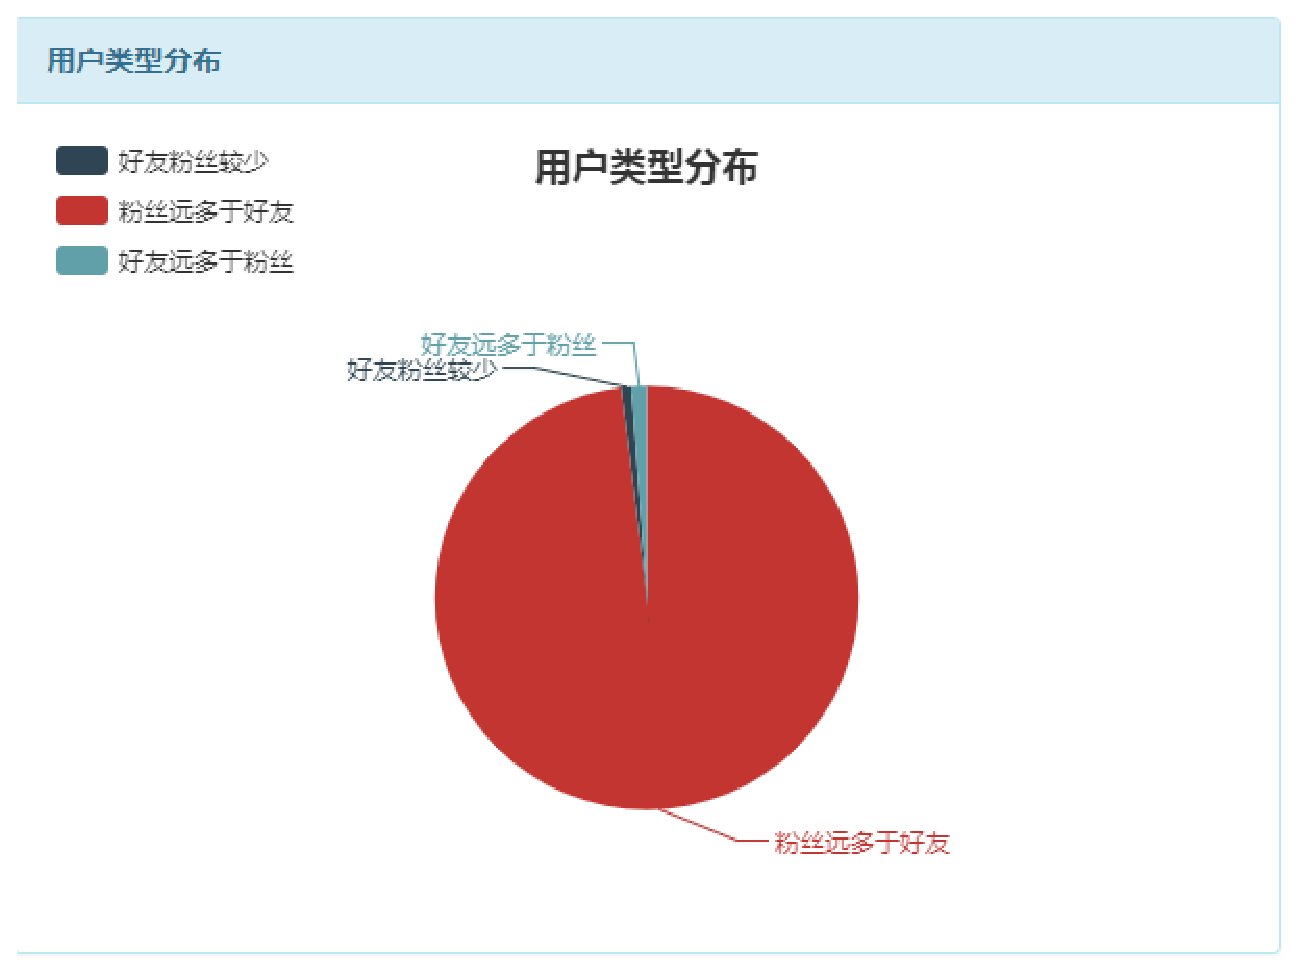
\includegraphics[width=0.15\textwidth]{IMAGE/group-images/44.eps}}
  \subfigure{
      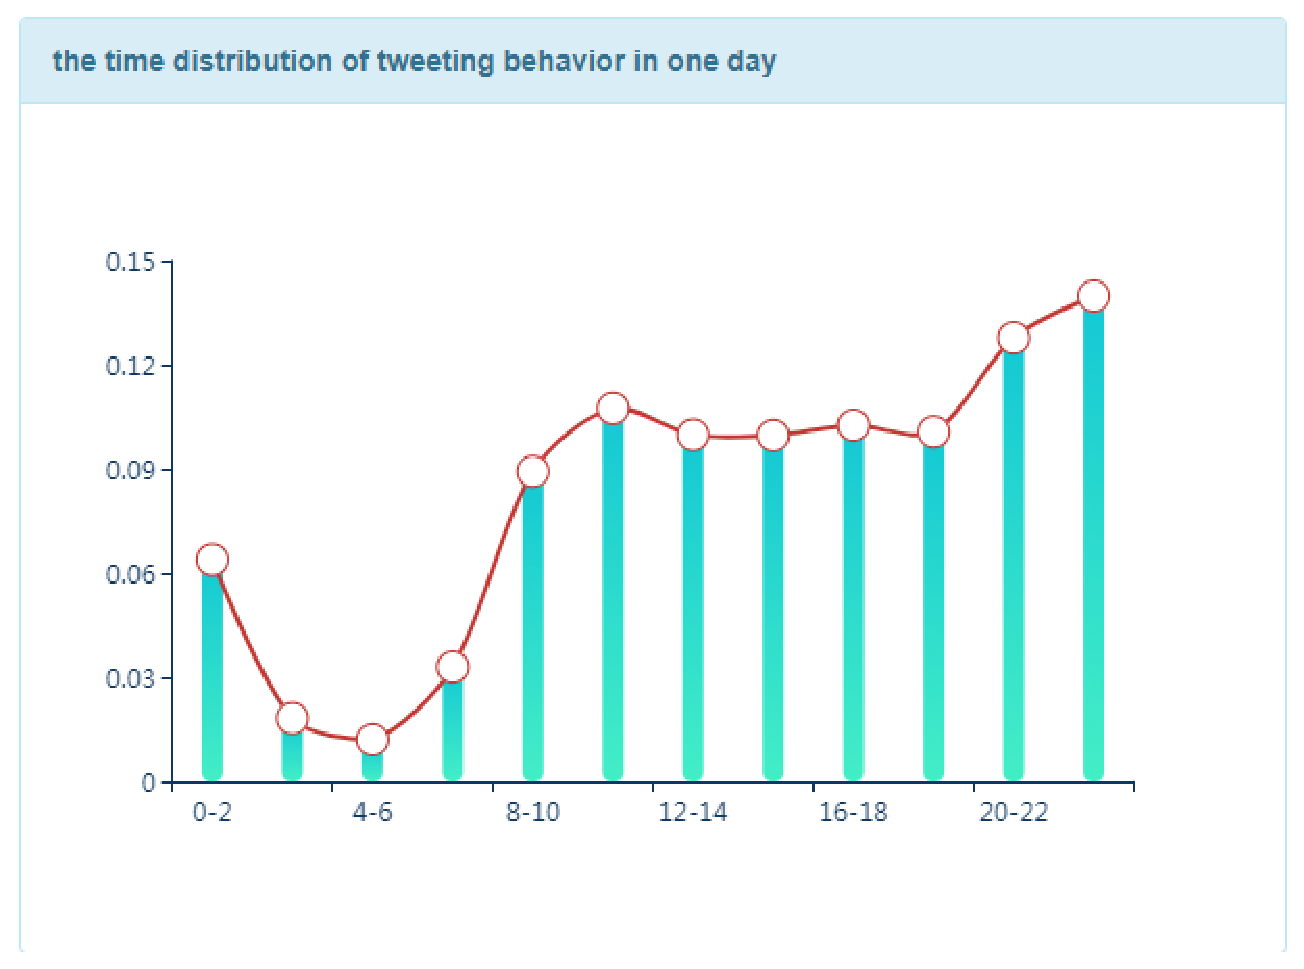
\includegraphics[width=0.15\textwidth]{IMAGE/group-images/45.eps}}
  \subfigure{
      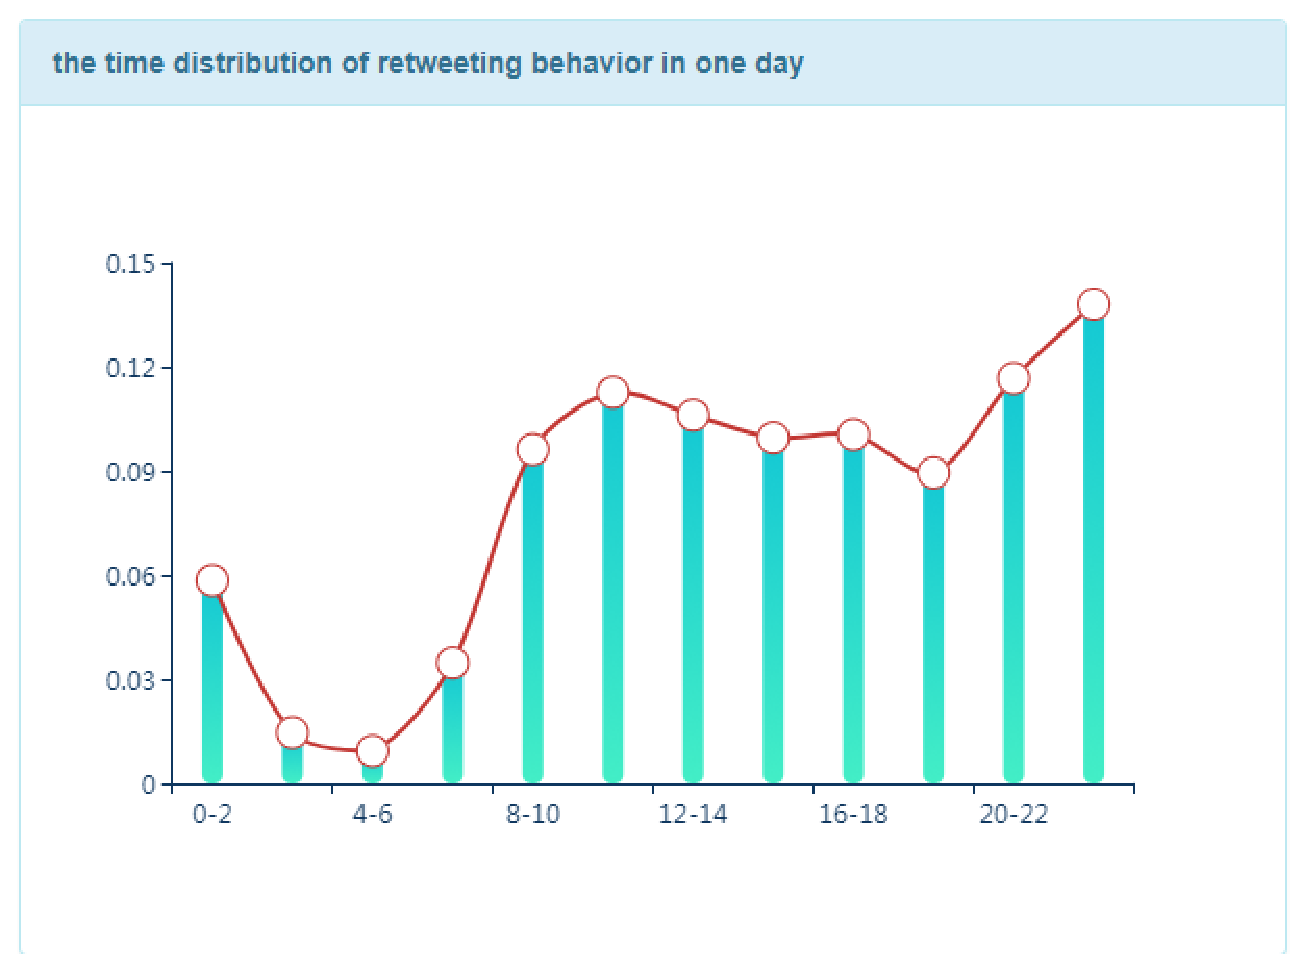
\includegraphics[width=0.15\textwidth]{IMAGE/group-images/46.eps}}
  \subfigure{
      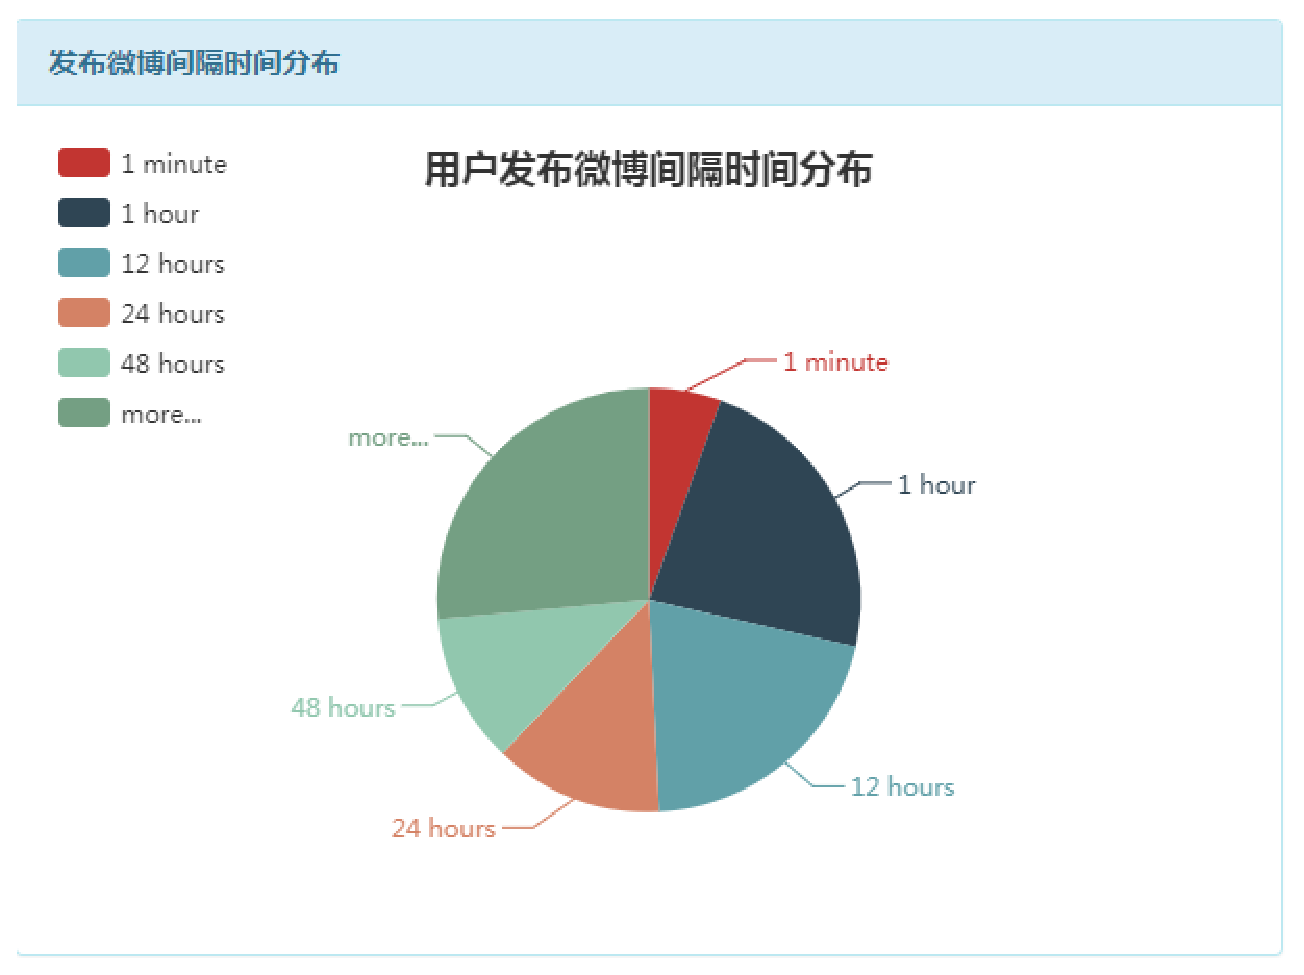
\includegraphics[width=0.15\textwidth]{IMAGE/group-images/47.eps}}
  \subfigure{
      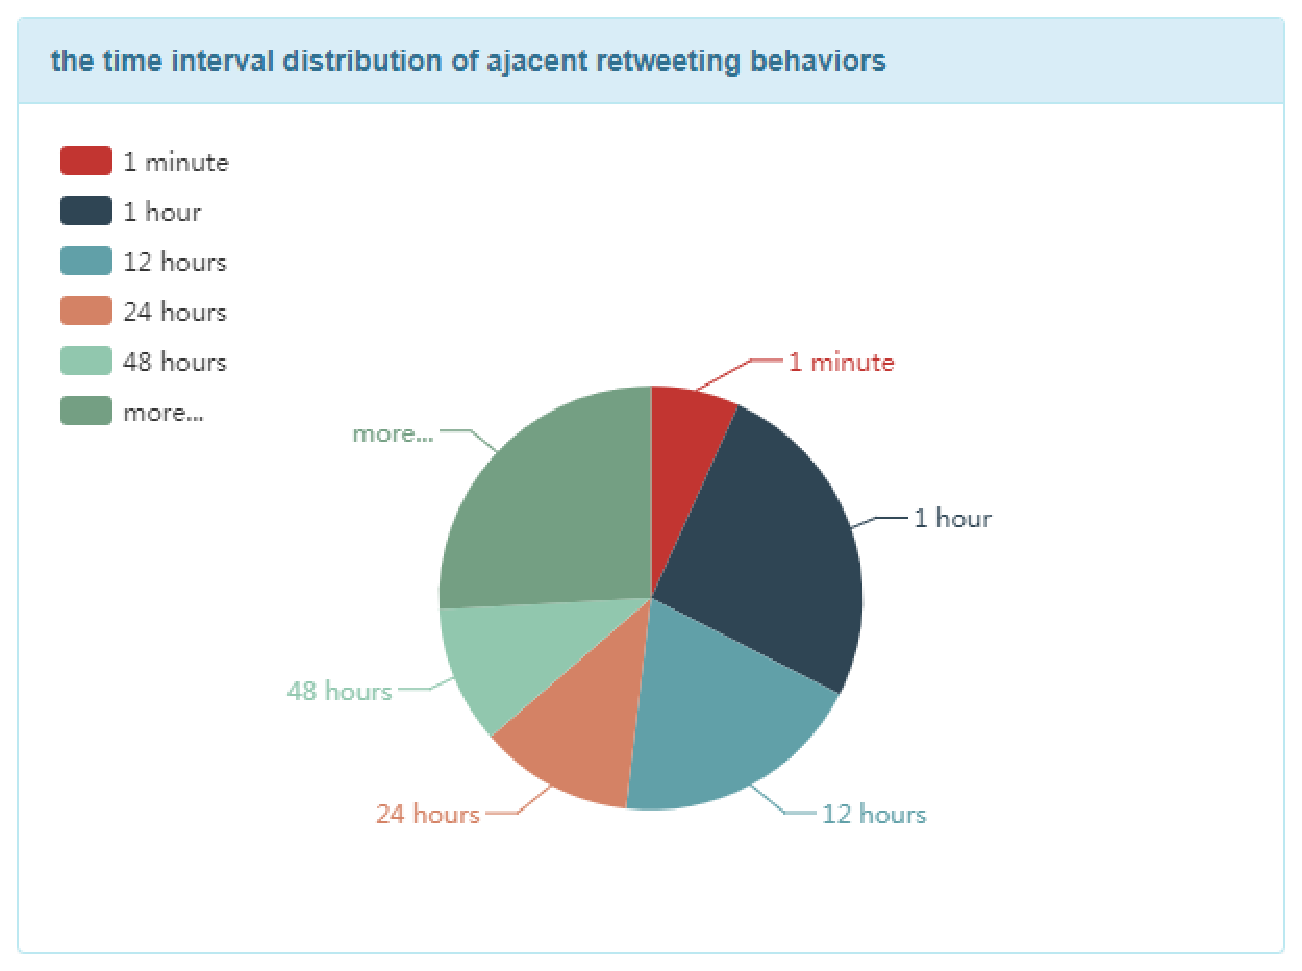
\includegraphics[width=0.15\textwidth]{IMAGE/group-images/48.eps}}
  \subfigure{
      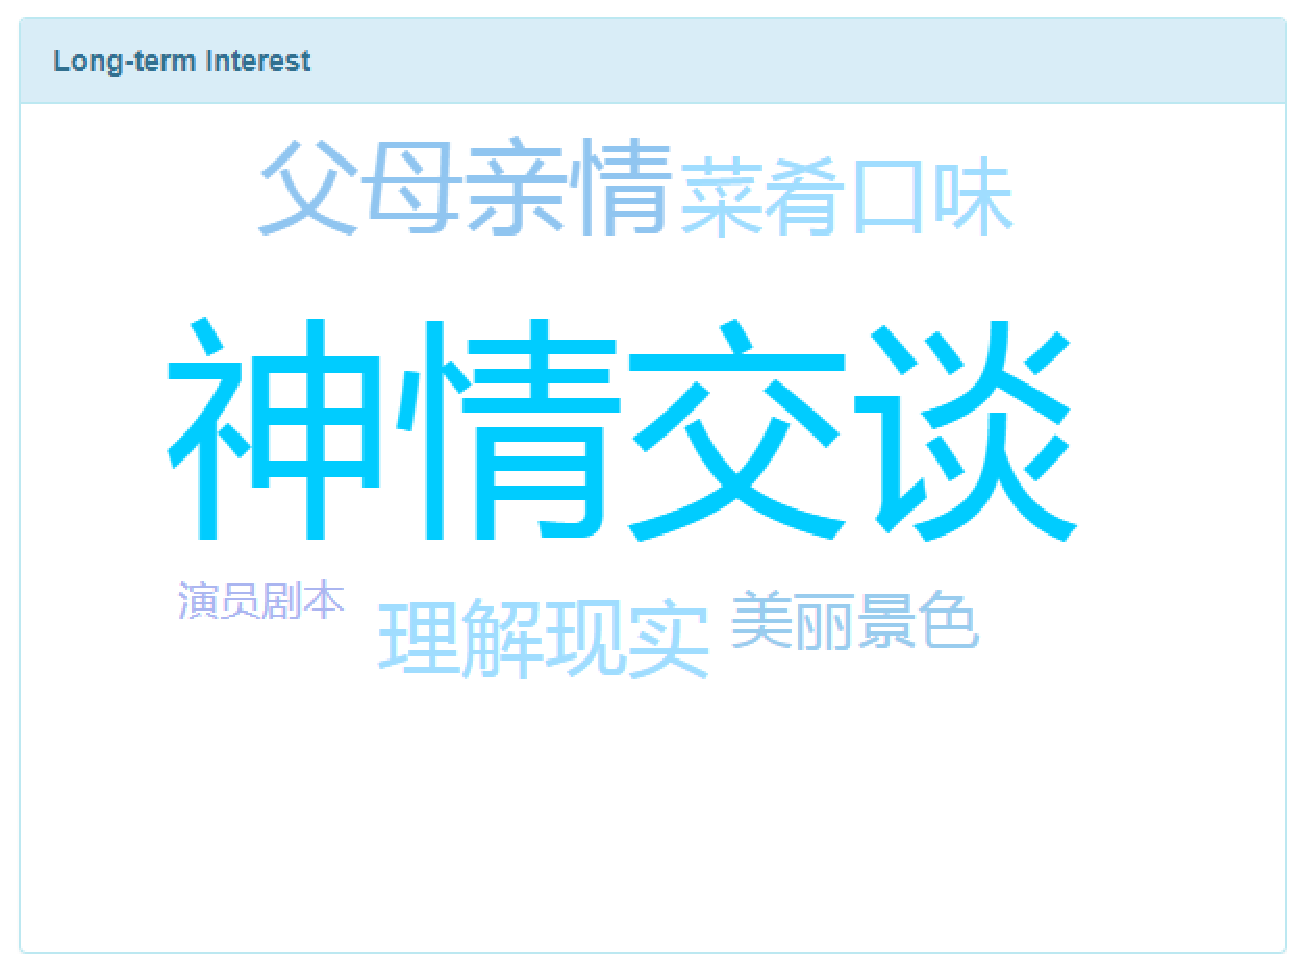
\includegraphics[width=0.15\textwidth]{IMAGE/group-images/49.eps}}
  \caption{The Statistics of User Group Four}
  \label{fig:subfig} %% label for entire figure
\end{figure}


\paragraph{Reposting Behavior Modeling}
By performing users clustering, we got four user groups. We generated instances by the method as described in subsection \ref{subsec:RepostingBehaviorPrediction}. However, we observed that positive instances (reposting) and negative instances (un-reposting) are much unbalanced. Thus we randomly select a subset of negative instances with the equal number of positive number for experiments. We compared our method with \cite{IEEEexample:conf/ijcai/ZhangLTCL13}, the results are list in figure \ref{fig:comparisons}, here we call our method as reposting model for group(RMG). The result suggests that our method had a better performance than LRC-BQ in most cases.\par

 \begin{figure}
  \centering
  \subfigure[Precision Of RMG	and LRC-BQ]{
    \label{fig:subfig:a} %% label for first subfigure
    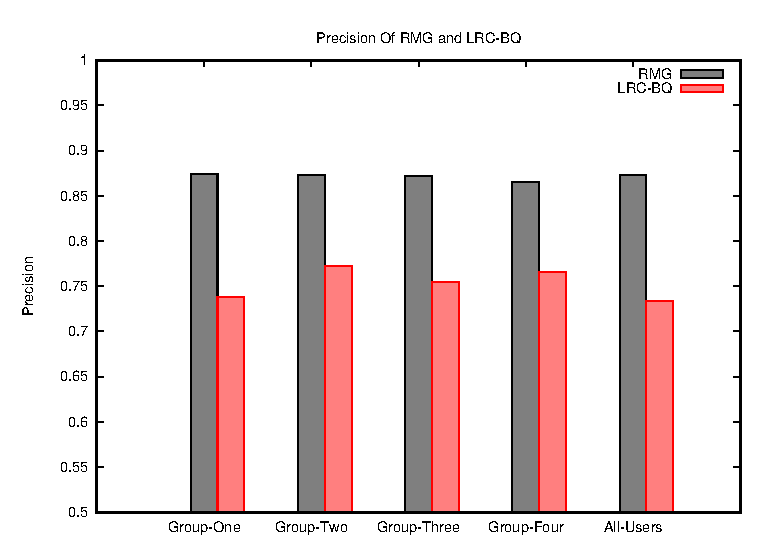
\includegraphics[width=0.4\textwidth]{IMAGE/model/precision.eps}}
  \hspace{1in}
  \subfigure[Recall Of RMG and LRC-BQ]{
    \label{fig:subfig:b} %% label for second subfigure
    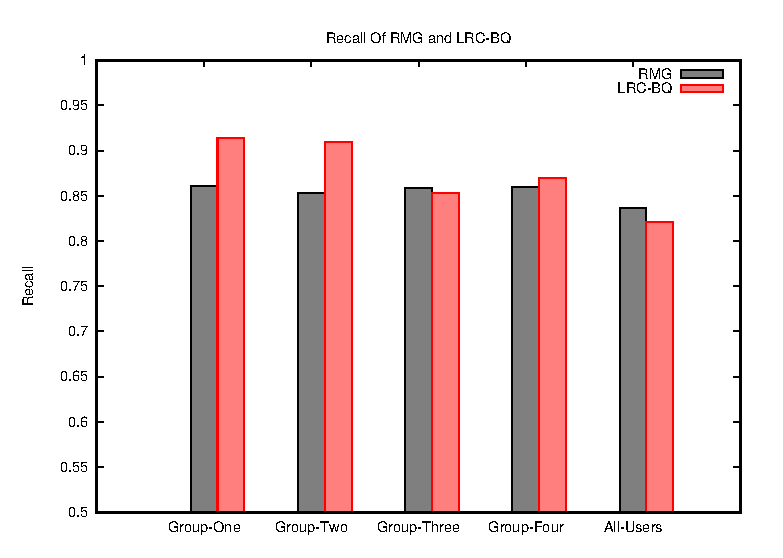
\includegraphics[width=0.4\textwidth]{IMAGE/model/recall.eps}}
  \hspace{1in}
  \subfigure[F-Measure Of RMG and LRC-BQ]{
    \label{fig:subfig:c} %% label for second subfigure
    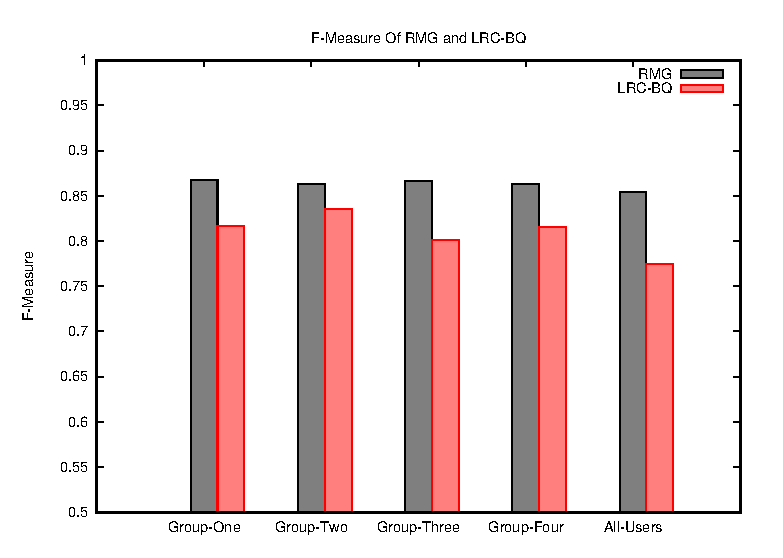
\includegraphics[width=0.4\textwidth]{IMAGE/model/F-Measure.eps}}
  \caption{Comparison Of RMG and LRC-BQ}
  \label{fig:comparisons} %% label for entire figure
\end{figure}


We further try different features and their combinations for modeling reposting behaviors, they are user-based information(UI), microblog-based information(MI), interaction information(II) and their combinations. The results are list in in figure \ref{fig:performances}. The result suggests that the MI and UI perform similarly for modeling group one and group three, MI performs better than UI and II on group four. Combining all the three types of features can get similar performance with the combination of UI and MI on group two and group three, and the two combinations perform better than all other combinations. As for group one and group four, using UI and MI can get the best performance, which indicates that there in deed exists strong correlation between the reposting behavior and the two types information.

 \begin{figure}
  \centering
  \subfigure[Precision of RMG Using Different Features]{
    \label{fig:subfig:a} %% label for first subfigure
    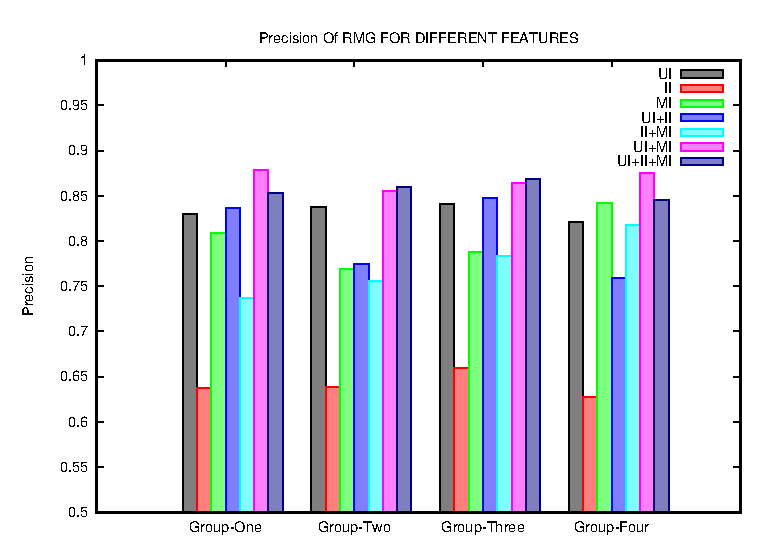
\includegraphics[width=0.4\textwidth]{IMAGE/model/precisionofdifferentfeatures.eps}}
  \hspace{1in}
  \subfigure[Recall of RMG Using Different Features]{
    \label{fig:subfig:b} %% label for second subfigure
    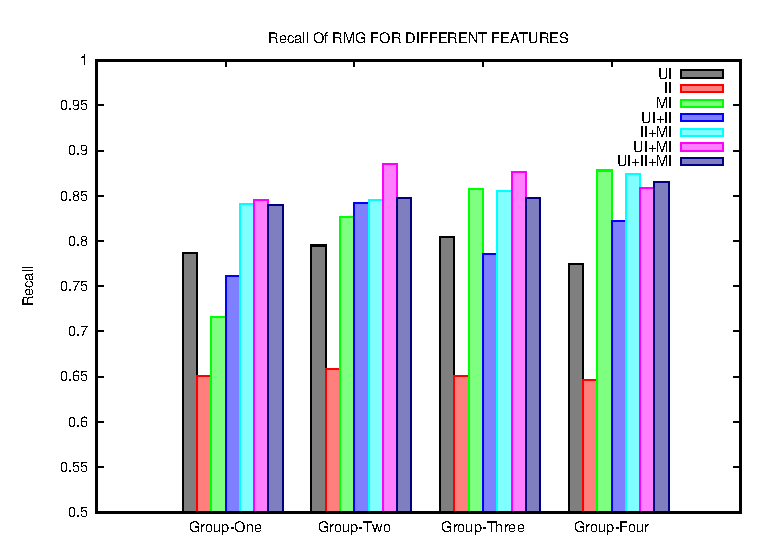
\includegraphics[width=0.4\textwidth]{IMAGE/model/recallofdifferentfeatures.eps}}
  \hspace{1in}
  \subfigure[F-Measure of RMG Using Different Features]{
    \label{fig:subfig:c} %% label for second subfigure
    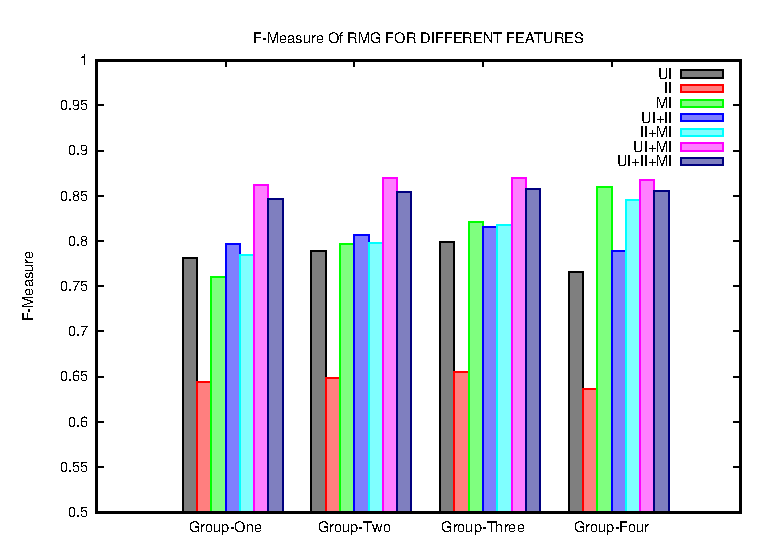
\includegraphics[width=0.4\textwidth]{IMAGE/model/fmeasureofdifferentfeatures.eps}}
  \caption{Performance Of RMG Using Different Features}
  \label{fig:performances} %% label for entire figure
\end{figure}

\paragraph{Time Report}
